\documentclass[a4paper,12pt]{article} % only 10 (default), 11 and 12 pt are available

% NECESSARY PACKAGES
\usepackage[utf8]{inputenc} % to be able to use non-English characters
\usepackage{amsmath}  % improve math presentation
\usepackage{physics}
\usepackage{amssymb}
\usepackage{xcolor}
\usepackage{float}
\usepackage{caption} % captioning package of wonders
\usepackage{url} % to incorporate clickable links
\usepackage{cite} % takes care of citations
\usepackage[final]{hyperref} % adds hyper links inside the generated PDF file

% NECESSARY FOR INCREASED CUSTOMIZATION PACKAGES
\usepackage{newfloat} % for defining new float in environments (e.g: figure and tables are floats)
\usepackage{graphicx} % takes care of graphic including machinery
\usepackage{tabularx} % extra features for tabular environment
\usepackage{array} % provides 'programmable' tables (cells can be tweaked much more)
\usepackage[export]{adjustbox} % to include boxed content other than figures (e.g: boxed equations)
\usepackage{wrapfig} % to make figures wrap around text
\usepackage{subcaption} % to make sub-figures inside of figures
\usepackage[spanish]{babel}
% TWEAKS FOR PACKAGES
\usepackage[margin=2cm,a4paper]{geometry} % tweaks margins
\captionsetup{justification=centering} % caption justification
\captionsetup{font=small} % caption text size
\captionsetup{labelfont=bf} % caption label font emphasis (e.g: 'Figure X:')
\numberwithin{equation}{section} % equations are named according to their section (e.g: 2.1)
\numberwithin{figure}{section} % figures are named according to their section (e.g: 3.4)
\hypersetup{
    colorlinks=true,      % false: boxed links; true: colored links
    linkcolor=black,      % color of internal links
    citecolor=blue,       % color of links to bibliography
    filecolor=magenta,    % color of file links
    urlcolor=red          % color of website links
}

\usepackage{lipsum} % DELETE THIS AND BELOW \lipsum[]'s AND YOU'RE GOOD TO GO

%++++++++++++++++++++++++++++++++++++++++++++++++++++++++++++++++++++++++++++++++

% HERE GOES THE COVER PAGE SETUP
%\newcommand{\hwcourse}{\text{Astrofísica Extragaláctica y Cosmología}} % Title of your document
\newcommand{\hwnumber}{\text{Diplomado Sismología} \\ \text{Uso de Datos Sismológicos}} % Name of your study number
\newcommand{\hwname}{\text{Actividad 3: Magnitudes}} % Name of your study name
\newcommand{\hwdetails}{ \text{Informe de resultados obtenidos} \\ 
                            \text{Tarea 3} \\ % Details about your study
                            \\\text{ }\\
                            \text{\textit{Red Sismológica Nacional de Colombia - Dirección de Geoamenazas}} }
%\newcommand{\hwdate}{\text{In case you want to add a date other than submission date}}
\newcommand{\hwauthor}{Keneth Garcia} % Your name or your group's names
\newcommand{\HRule}{\rule{\linewidth}{0.5mm}} % line widths in the cover page

%++++++++++++++++++++++++++++++++++++++++++++++++++++++++++++++++++++++++++++++++

\begin{document}

% COVER PAGE IS COMPILED HERE
\begin{titlepage}
\begin{center} % Center remainder of the page
% LOGO SECTION

\includegraphics[width = 8cm]{Figures/sgc_logo}
\\[3cm]

% HEADING SECTIONS
\textsc{\LARGE Servicio Geológico Colombiano}\\[.5cm]
\textsc{\Large Universidad de Chile}\\[1.5cm]

% TITLE SECTION
\HRule \\[0.4cm]
%{ \huge \bfseries \hwcourse}\\ \vspace{.5cm} 
{ \huge \bfseries \hwnumber}\\ \vspace{.5cm} 
{ \large \bfseries \hwname}\\ \vspace{.5cm} 
{ \hwdetails}\\ \vspace{.5cm}
%{ \bfseries \hwdate}\\ \vspace{.5cm} 
\HRule \\[1.5cm]
\end{center} 

% AUTHOR SECTION
\begin{flushleft} % left oriented author section
    \large 
    \textit{Escrito por:}\\
    \hwauthor% Your name
\end{flushleft}
\vspace{5cm}
\makeatletter
Fecha: \today % \@date 
\vfill % Fill the rest of the page with white space
\makeatother
\end{titlepage}

%++++++++++++++++++++++++++++++++++++++++++++++++++++++++++++++++++++++++++++++++

\newpage

%\tableofcontents

%\newpage

%\begin{abstract}
    %\lipsum[1]
%\end{abstract}

%\newpage
\section{Introducción}

La determinación de la magnitud de un terremoto constituye una etapa fundamental para caracterizar su tamaño y comparar de manera objetiva eventos sísmicos registrados en distintos contextos tectónicos y a diferentes distancias de las estaciones de observación. La magnitud no corresponde a una medida directa del daño producido ni de la percepción de la población, sino a una estimación cuantitativa basada en parámetros físicos medidos sobre los registros sísmicos, tales como la amplitud máxima de la señal o el nivel de baja frecuencia de su espectro de desplazamiento.

En esta actividad se estiman la magnitud local, \(M_L\), y la magnitud de momento, \(M_w\), de un evento ocurrido en el norte de Chile, cuyo hipocentro se encuentra definido por una latitud de \(-20{,}12^\circ\), una longitud de \(-69{,}33^\circ\) y una profundidad de \(90\)~km. El análisis se realiza utilizando registros de cinco estaciones sismológicas: MNMCX, PATA, PSGCX, UNAP y PB07. Para cada estación se dispone de sus coordenadas, distancia epicentral y registros de las componentes horizontales y verticales de la señal sísmica.[272]

La magnitud local \(M_L\) se calcula a partir de sismogramas sintéticos Wood--Anderson, utilizando la amplitud máxima observada en las componentes horizontales y una corrección dependiente de la distancia epicentral. Este procedimiento representa una aplicación de la metodología clásica de magnitud local, en la cual la amplitud medida debe expresarse en milímetros y ser ajustada según la distancia entre la estación y el epicentro. La estimación final de \(M_L\) se obtiene a partir del promedio de las magnitudes calculadas en las componentes horizontales de cada estación y, posteriormente, del promedio entre estaciones.

Por otro lado, la magnitud de momento \(M_w\) se estima mediante análisis espectral de los registros de desplazamiento. Para ello, se selecciona una ventana temporal representativa de la onda S en cada estación y se calcula el espectro de amplitud de las componentes este--oeste, norte--sur y vertical. El parámetro principal corresponde al plateau de baja frecuencia del espectro de desplazamiento, el cual está relacionado con el momento sísmico escalar \(M_0\). A partir de los valores de plateau, la distancia hipocentral, la densidad y la velocidad de onda S en las cercanías de la fuente, se obtiene el momento sísmico y posteriormente la magnitud de momento.

El cálculo conjunto de \(M_L\) y \(M_w\) permite comparar dos aproximaciones que describen el tamaño de un mismo evento a partir de observables diferentes. Mientras \(M_L\) depende de la amplitud máxima registrada por un instrumento Wood--Anderson y de una corrección por distancia, \(M_w\) se fundamenta en el momento sísmico y en el comportamiento de baja frecuencia del espectro de desplazamiento. Esta diferencia metodológica permite discutir la consistencia entre ambas estimaciones, las limitaciones asociadas a la selección de amplitudes y ventanas espectrales, y la influencia de la geometría fuente--estación y de las propiedades físicas asumidas para el medio de propagación.

El presente documento presenta los resultados obtenidos durante el desarrollo de la actividad de determinación de magnitudes. La sección de metodología describe los datos utilizados, los parámetros físicos adoptados, el procedimiento para estimar \(M_L\) a partir de las amplitudes Wood--Anderson y el análisis espectral aplicado para calcular \(M_w\). La sección de resultados presenta las amplitudes máximas, los plateaus espectrales, las estimaciones de magnitud por componente y por estación, así como los valores promedio finales. Posteriormente, la sección de discusión compara las metodologías de magnitud local y magnitud de momento, diferencia los conceptos de magnitud e intensidad y analiza las posibles causas de similitudes o discrepancias entre los resultados. Finalmente, la sección de conclusiones sintetiza los principales hallazgos, las limitaciones del análisis y la interpretación general de las magnitudes obtenidas.
\newpage

\section{Metodología}

Para la estimación de las magnitudes se emplearon registros de cinco estaciones sismológicas: MNMCX, PATA, PSGCX, UNAP y PB07. El evento analizado posee una localización hipocentral previamente definida, con coordenadas \((-20{,}12^\circ,\,-69{,}33^\circ)\) y una profundidad de \(90~\mathrm{km}\). Se utilizaron las distancias epicentrales entregadas para cada estación y dos conjuntos de registros: sismogramas sintéticos Wood--Anderson para el cálculo de \(M_L\), y sismogramas de desplazamiento para el cálculo de \(M_w\).

Los datos se procesaron mediante notebooks desarrollados en Python, utilizando principalmente las bibliotecas \texttt{NumPy}, \texttt{Pandas}, \texttt{Matplotlib} y \texttt{SciPy}. Previamente a los cálculos, se verificó la disponibilidad de los archivos correspondientes a cada estación y componente, se revisaron las series temporales y se controló visualmente que las señales utilizadas contuvieran el evento y presentaran características adecuadas para cada método de estimación.

\subsection{Cálculo de magnitud local \(M_L\)}

La magnitud local se estimó utilizando los sismogramas sintéticos Wood--Anderson almacenados en la carpeta \texttt{DatosWA}. Los registros se encontraban expresados en desplazamiento físico, en unidades de metros, y se utilizaron exclusivamente las componentes horizontales este--oeste (\texttt{HHE}) y norte--sur (\texttt{HHN}) de cada estación. La componente vertical no se incorporó en este cálculo, de acuerdo con la definición utilizada para la magnitud local.

En primer lugar, se cargaron automáticamente todas las trazas horizontales disponibles y se generaron gráficos de cada señal para verificar la presencia del paquete de ondas asociado al evento, la calidad general del registro y la ubicación temporal de las amplitudes máximas. Para cada componente se determinó la amplitud máxima absoluta de desplazamiento mediante:

\[
A_{\max} = \max \left|u(t)\right|,
\]

donde \(u(t)\) corresponde a la amplitud de la traza Wood--Anderson en función del tiempo.
El algoritmo diseñado identificó el máximo absoluto de cada registro y se generaron figuras de control en las que se resaltó la zona temporal que contiene dicho máximo. Esta revisión permitió verificar que el valor seleccionado correspondiera a la señal sísmica y no a ruido o a una oscilación no representativa.

Las amplitudes obtenidas inicialmente en metros fueron convertidas a milímetros, pues esta es la unidad requerida en la formulación de la magnitud local:

\[
A_{\mathrm{mm}} = 1000 A_{\mathrm{m}}.
\]

Para cada estación y componente horizontal se calculó la corrección de distancia utilizando la distancia epicentral \(\Delta\), expresada en kilómetros:

\[
-\log_{10}(A_0) =
\log_{10}\left(\frac{\Delta}{100}\right)+3.
\]

Posteriormente, la magnitud local por componente se obtuvo mediante:

\[
M_L =
\log_{10}\left(A_{\mathrm{mm}}\right)
+
\log_{10}\left(\frac{\Delta}{100}\right)
+
3.
\]

Y se calculó una magnitud para cada componente horizontal, \(M_{L,E}\) y \(M_{L,N}\), obteniendo una magnitud representativa por estación mediante el promedio:

\[
M_{L,\mathrm{estación}} =
\frac{M_{L,E}+M_{L,N}}{2}.
\]

Finalmente, la magnitud local del evento se estimó a partir del promedio aritmético de las magnitudes obtenidas en las cinco estaciones:

\[
\overline{M_L} =
\frac{1}{N}
\sum_{i=1}^{N}M_{L,i},
\]

donde \(N\) corresponde al número de estaciones con estimaciones válidas. Como medida de dispersión se calcularon la desviación estándar muestral entre estaciones y el error estándar de la media:

\[
\mathrm{SEM}_{M_L} =
\frac{s_{M_L}}{\sqrt{N}}.
\]

\subsection{Cálculo de magnitud de momento \(M_w\)}

La magnitud de momento se estimó mediante análisis espectral de los registros de desplazamiento contenidos en la carpeta \texttt{DatosInt}. Para cada una de las cinco estaciones se utilizaron las tres componentes disponibles: este--oeste (\texttt{HHE}), norte--sur (\texttt{HHN}) y vertical (\texttt{HHZ}). Los archivos fueron cargados automáticamente a partir de sus nombres, identificando la red, estación y componente correspondiente.

Como primer paso, se generaron gráficos de las tres componentes de cada estación para identificar visualmente la llegada de la onda S. Para cada estación se definió manualmente una ventana temporal que incluyera la fase S y una parte de su coda temprana. La misma ventana se aplicó de manera consistente a las tres componentes de una estación. La selección de la ventana excluyó, en lo posible, la fase P y los segmentos tardíos donde la señal estuviera dominada por ruido.

A cada ventana de onda S se le removió la media y la tendencia lineal mediante la función \texttt{signal.detrend} de \texttt{SciPy}. Posteriormente, se calculó la transformada rápida de Fourier usando:

\[
U(f) =
\frac{\mathrm{FFT}[u(t)]}{N_s},
\]

donde \(N_s\) corresponde al número de muestras de la ventana S seleccionada. La normalización por el número de muestras permite comparar las amplitudes espectrales entre ventanas de distinta duración. Para obtener el espectro unilateral, las amplitudes de las frecuencias internas fueron multiplicadas por un factor de dos, manteniendo sin modificación la componente de frecuencia cero y, cuando corresponde, la frecuencia de Nyquist.

A partir de los espectros de amplitud de desplazamiento se identificó, para cada estación, una banda de baja frecuencia aproximadamente plana. Esta región corresponde al plateau espectral \(\Omega_0\), asociado al momento sísmico. La selección de la banda se realizó visualmente sobre gráficos logarítmicos de frecuencia versus amplitud espectral, evitando la frecuencia cero, los primeros bins afectados por tendencia residual o duración finita de la ventana, los picos espectrales aislados y el tramo posterior a la frecuencia de esquina, donde se observa el decaimiento de la amplitud con la frecuencia.

Para cada componente se calculó el plateau como el promedio aritmético de las amplitudes espectrales dentro de la banda seleccionada:

\[
\Omega_{E}, \qquad
\Omega_{N}, \qquad
\Omega_{Z}.
\]

Los valores de las tres componentes se combinaron mediante una media cuadrática:

\[
\Omega_{\mathrm{RMS}} =
\left(
\frac{
\Omega_E^2+\Omega_N^2+\Omega_Z^2
}{3}
\right)^{1/2}.
\]

La distancia fuente--estación utilizada en el cálculo corresponde a la distancia hipocentral \(R\), obtenida a partir de la distancia epicentral y la profundidad conocida del evento:

\[
R =
\sqrt{\Delta^2+h^2}.
\]

Para mantener la consistencia dimensional, la distancia se convirtió de kilómetros a metros, la densidad se convirtió de \(\mathrm{g/cm^3}\) a \(\mathrm{kg/m^3}\), y la velocidad de onda S se convirtió de \(\mathrm{km/s}\) a \(\mathrm{m/s}\). Se utilizaron los parámetros físicos establecidos para la actividad:

\[
V = 2,
\]

\[
\left< R_S \right> = 0{,}67,
\]

\[
\rho = 3380~\mathrm{kg/m^3},
\]

\[
\beta = 4780~\mathrm{m/s}.
\]

El momento sísmico escalar por estación se calculó con la expresión:

\[
M_0 =  \frac{4\pi\rho\beta^3R}{ V\langle R_S \rangle } \Omega_{\mathrm{RMS}}.
\]

Finalmente, la magnitud de momento por estación se obtuvo mediante:

\[
M_w =
\frac{2}{3}\log_{10}(M_0)-6{,}07,
\]

donde \(M_0\) se expresa en \(\mathrm{N\,m}\). La magnitud de momento final del evento se determinó como el promedio de las estimaciones individuales de las estaciones:

\[
\overline{M_w} =
\frac{1}{N}
\sum_{i=1}^{N}M_{w,i}.
\]

Asimismo, se calcularon la desviación estándar entre estaciones y el error estándar de la media, con el propósito de cuantificar la dispersión estadística de las estimaciones obtenidas.
\newpage






\section{Resultados}

\subsection{Resultados de magnitud local \(M_L\)}

\begin{table}[htb]
    \centering
    \caption{Resumen de las trazas Wood--Anderson horizontales utilizadas para el cálculo de la magnitud local. Todas las señales presentan 17001 muestras y una duración de 170~s.}
    \label{tab:trazas-wa}
    \begin{tabular}{l l l l r r}
        \hline
        Estación & Componente & Red & Archivo & Muestras & Duración [s] \\
        \hline
        MNMCX & HHE & CX & \texttt{CX.MNMCX..HHE.dat} & 17001 & 170.0 \\
        MNMCX & HHN & CX & \texttt{CX.MNMCX..HHN.dat} & 17001 & 170.0 \\
        PATA  & HHE & IQ & \texttt{IQ.PATA..HHE.dat}  & 17001 & 170.0 \\
        PATA  & HHN & IQ & \texttt{IQ.PATA..HHN.dat}  & 17001 & 170.0 \\
        PB07  & HHE & CX & \texttt{CX.PB07..HHE.dat} & 17001 & 170.0 \\
        PB07  & HHN & CX & \texttt{CX.PB07..HHN.dat} & 17001 & 170.0 \\
        PSGCX & HHE & CX & \texttt{CX.PSGCX..HHE.dat} & 17001 & 170.0 \\
        PSGCX & HHN & CX & \texttt{CX.PSGCX..HHN.dat} & 17001 & 170.0 \\
        UNAP  & HHE & IQ & \texttt{IQ.UNAP..HHE.dat} & 17001 & 170.0 \\
        UNAP  & HHN & IQ & \texttt{IQ.UNAP..HHN.dat} & 17001 & 170.0 \\
        \hline
    \end{tabular}
\end{table}

Para el cálculo de la magnitud local se utilizaron diez trazas Wood--Anderson, correspondientes a las dos componentes horizontales, este--oeste (\texttt{HHE}) y norte--sur (\texttt{HHN}) de las cinco estaciones consideradas. Las estaciones MNMCX, PB07 y PSGCX pertenecen a la red \texttt{CX}, mientras que PATA y UNAP pertenecen a la red \texttt{IQ}. Cada traza contiene 17001 muestras y tiene una duración total de 170~s, lo cual permite identificar el paquete de ondas asociado al evento y determinar la amplitud máxima de cada componente (\ref{tab:trazas-wa}).

La Figura~\ref{fig:trazas-wa-horizontales} muestra las señales Wood--Anderson disponibles para las cinco estaciones. Cada panel corresponde a una componente horizontal y presenta la amplitud en metros en función del tiempo. La visualización conjunta permite reconocer la variabilidad de la respuesta registrada entre estaciones, así como la presencia de los principales paquetes de ondas asociados al evento. Además, esta inspección permitió verificar que los registros contaban con información adecuada para aplicar la detección automática de amplitudes máximas.

\begin{figure}[htbp]
    \centering
    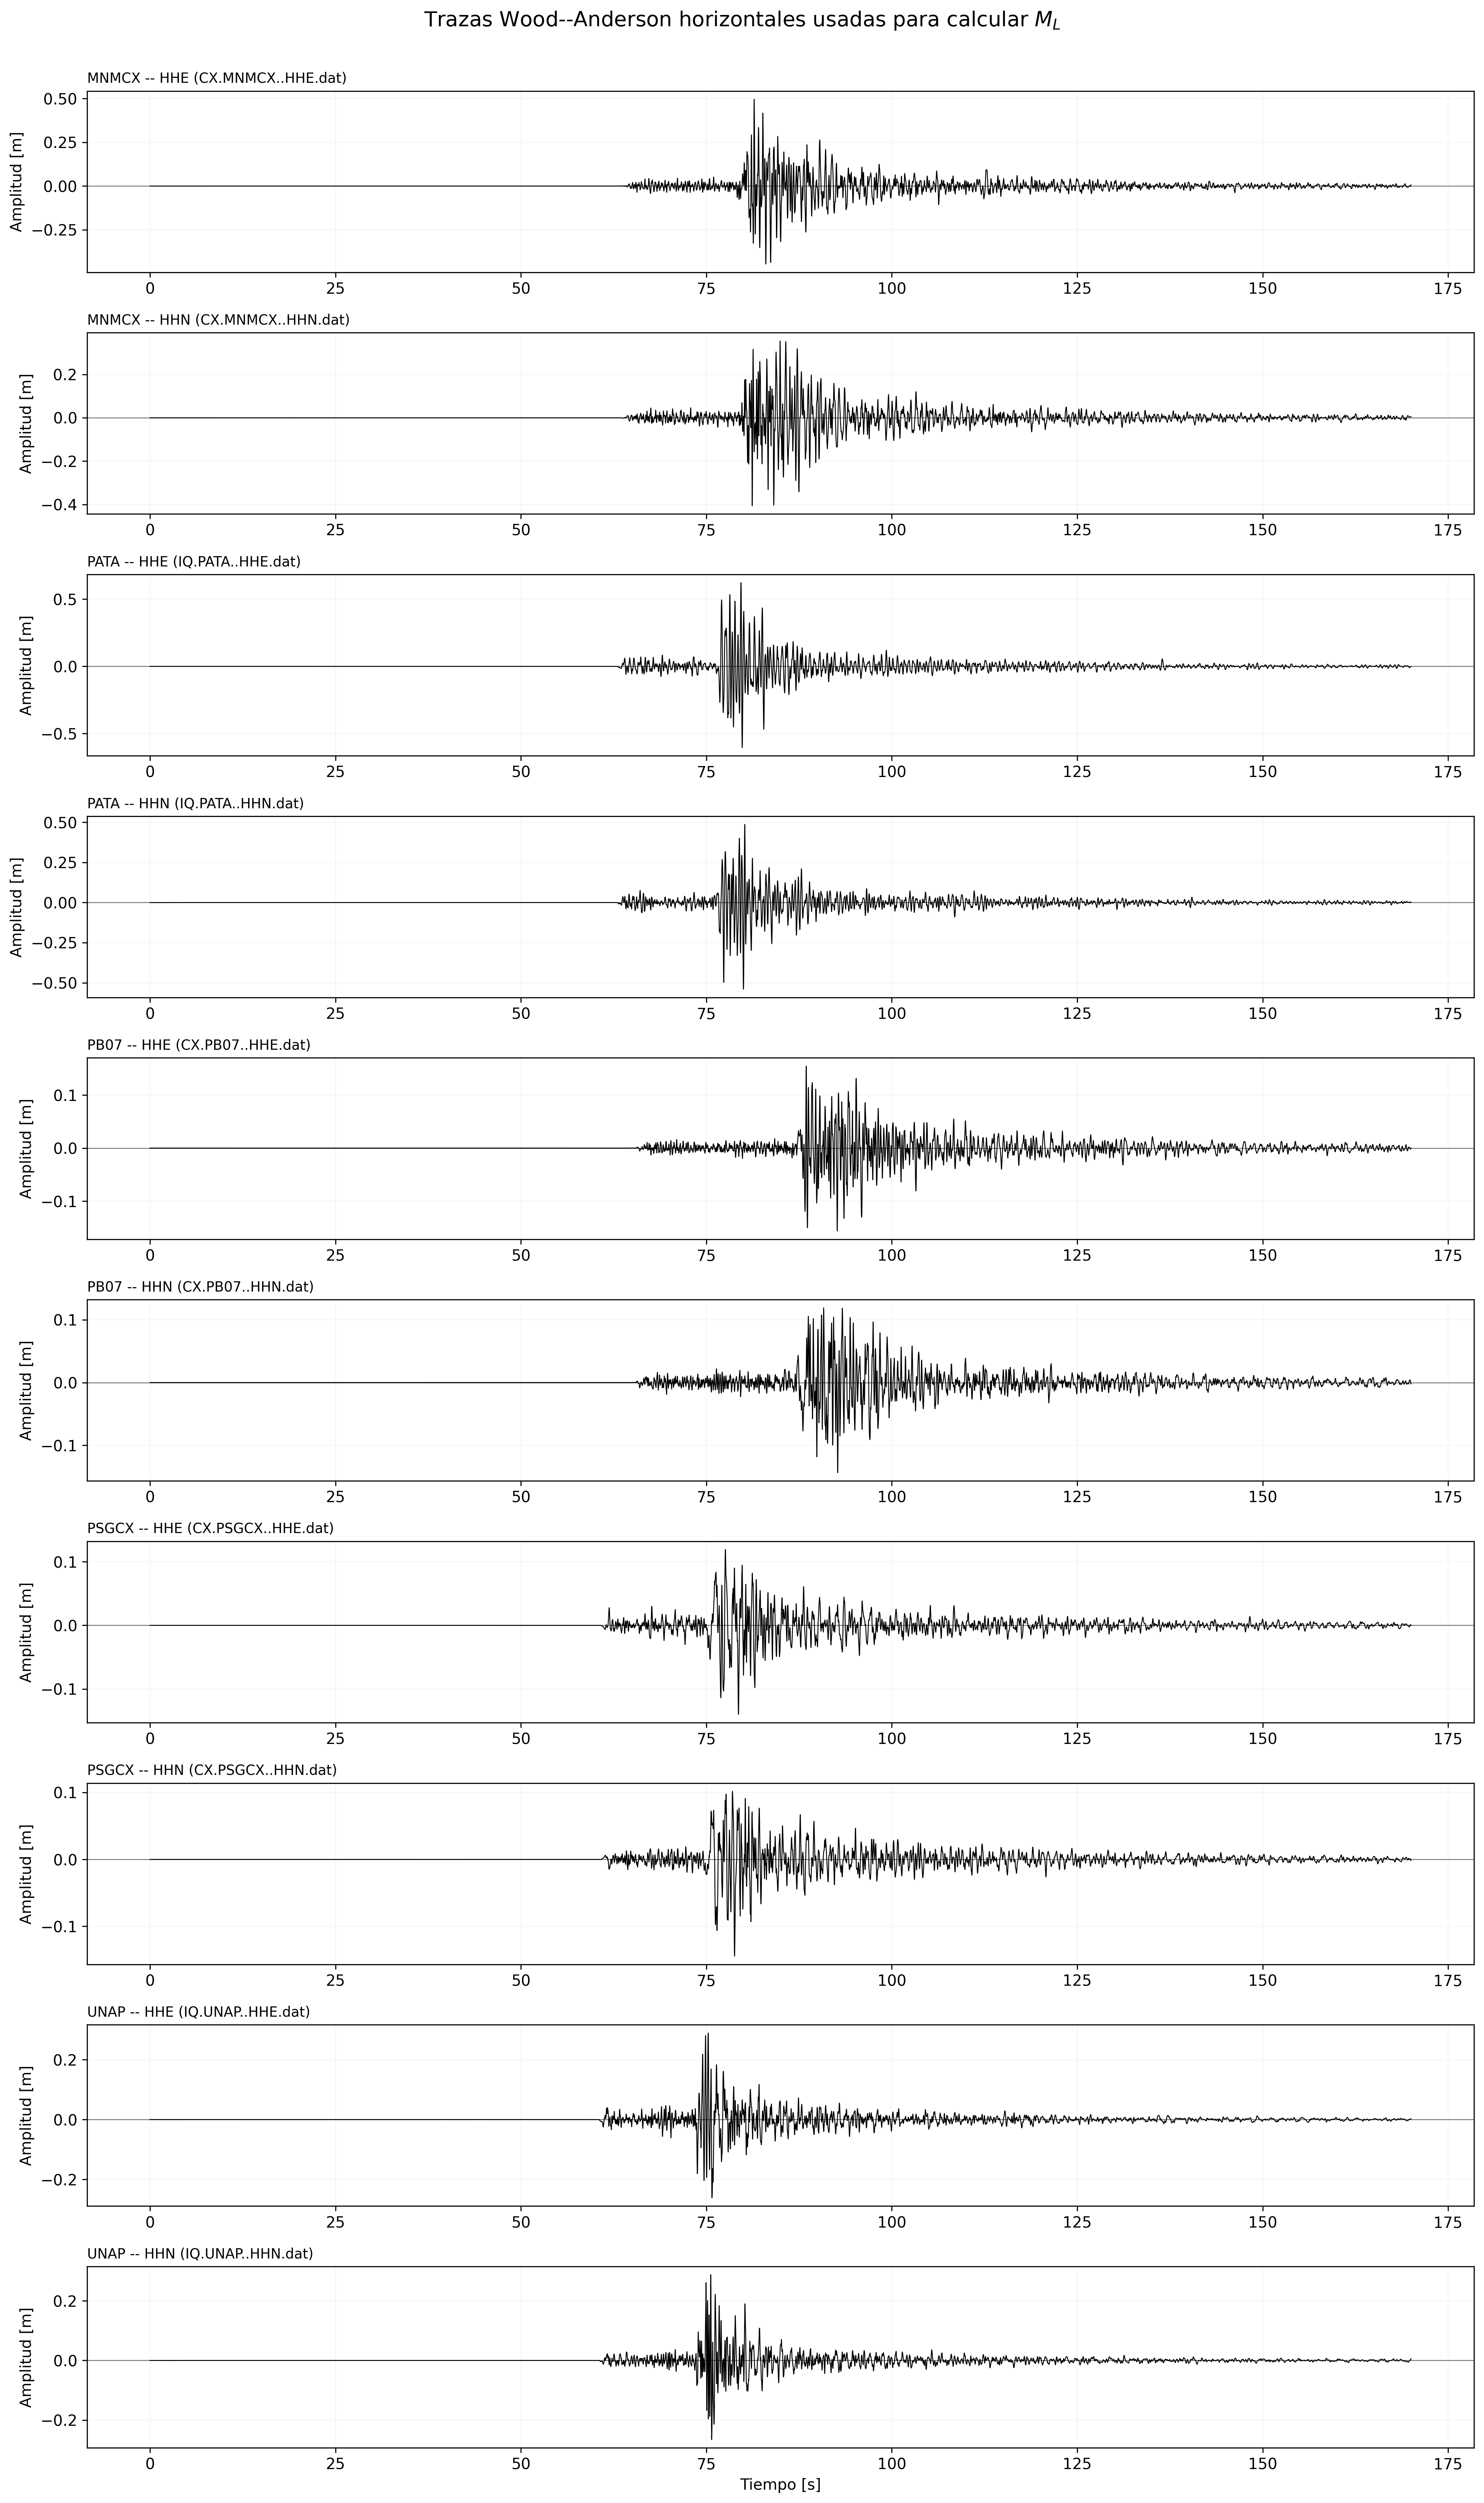
\includegraphics[width=0.75 \textwidth]{Figures/trazas_wa_horizontales}
    \caption{Trazas Wood--Anderson horizontales utilizadas para el cálculo de la magnitud local. Se presentan las componentes HHE y HHN de las estaciones MNMCX, PATA, PB07, PSGCX y UNAP. Las señales están expresadas en desplazamiento físico, en metros.}
    \label{fig:trazas-wa-horizontales}
\end{figure}

La amplitud máxima absoluta de cada señal se determinó mediante el criterio:

\[
A_{\max} = \max\left|u(t)\right|,
\]

donde \(u(t)\) representa la amplitud Wood--Anderson en función del tiempo. La Figura~\ref{fig:amplitud-maxima-automatica} presenta un ejemplo del procedimiento para la componente HHE de la estación MNMCX. La franja amarilla corresponde a una ventana de inspección centrada en la máxima amplitud identificada automáticamente, mientras que el marcador rojo indica la muestra donde se alcanza dicho máximo. Para este ejemplo, la amplitud máxima corresponde a \(0{,}496529~\mathrm{m}\), equivalente a \(496{,}529~\mathrm{mm}\), y se encuentra a los \(81{,}44~\mathrm{s}\) del registro.

\begin{figure}[htbp]
    \centering
    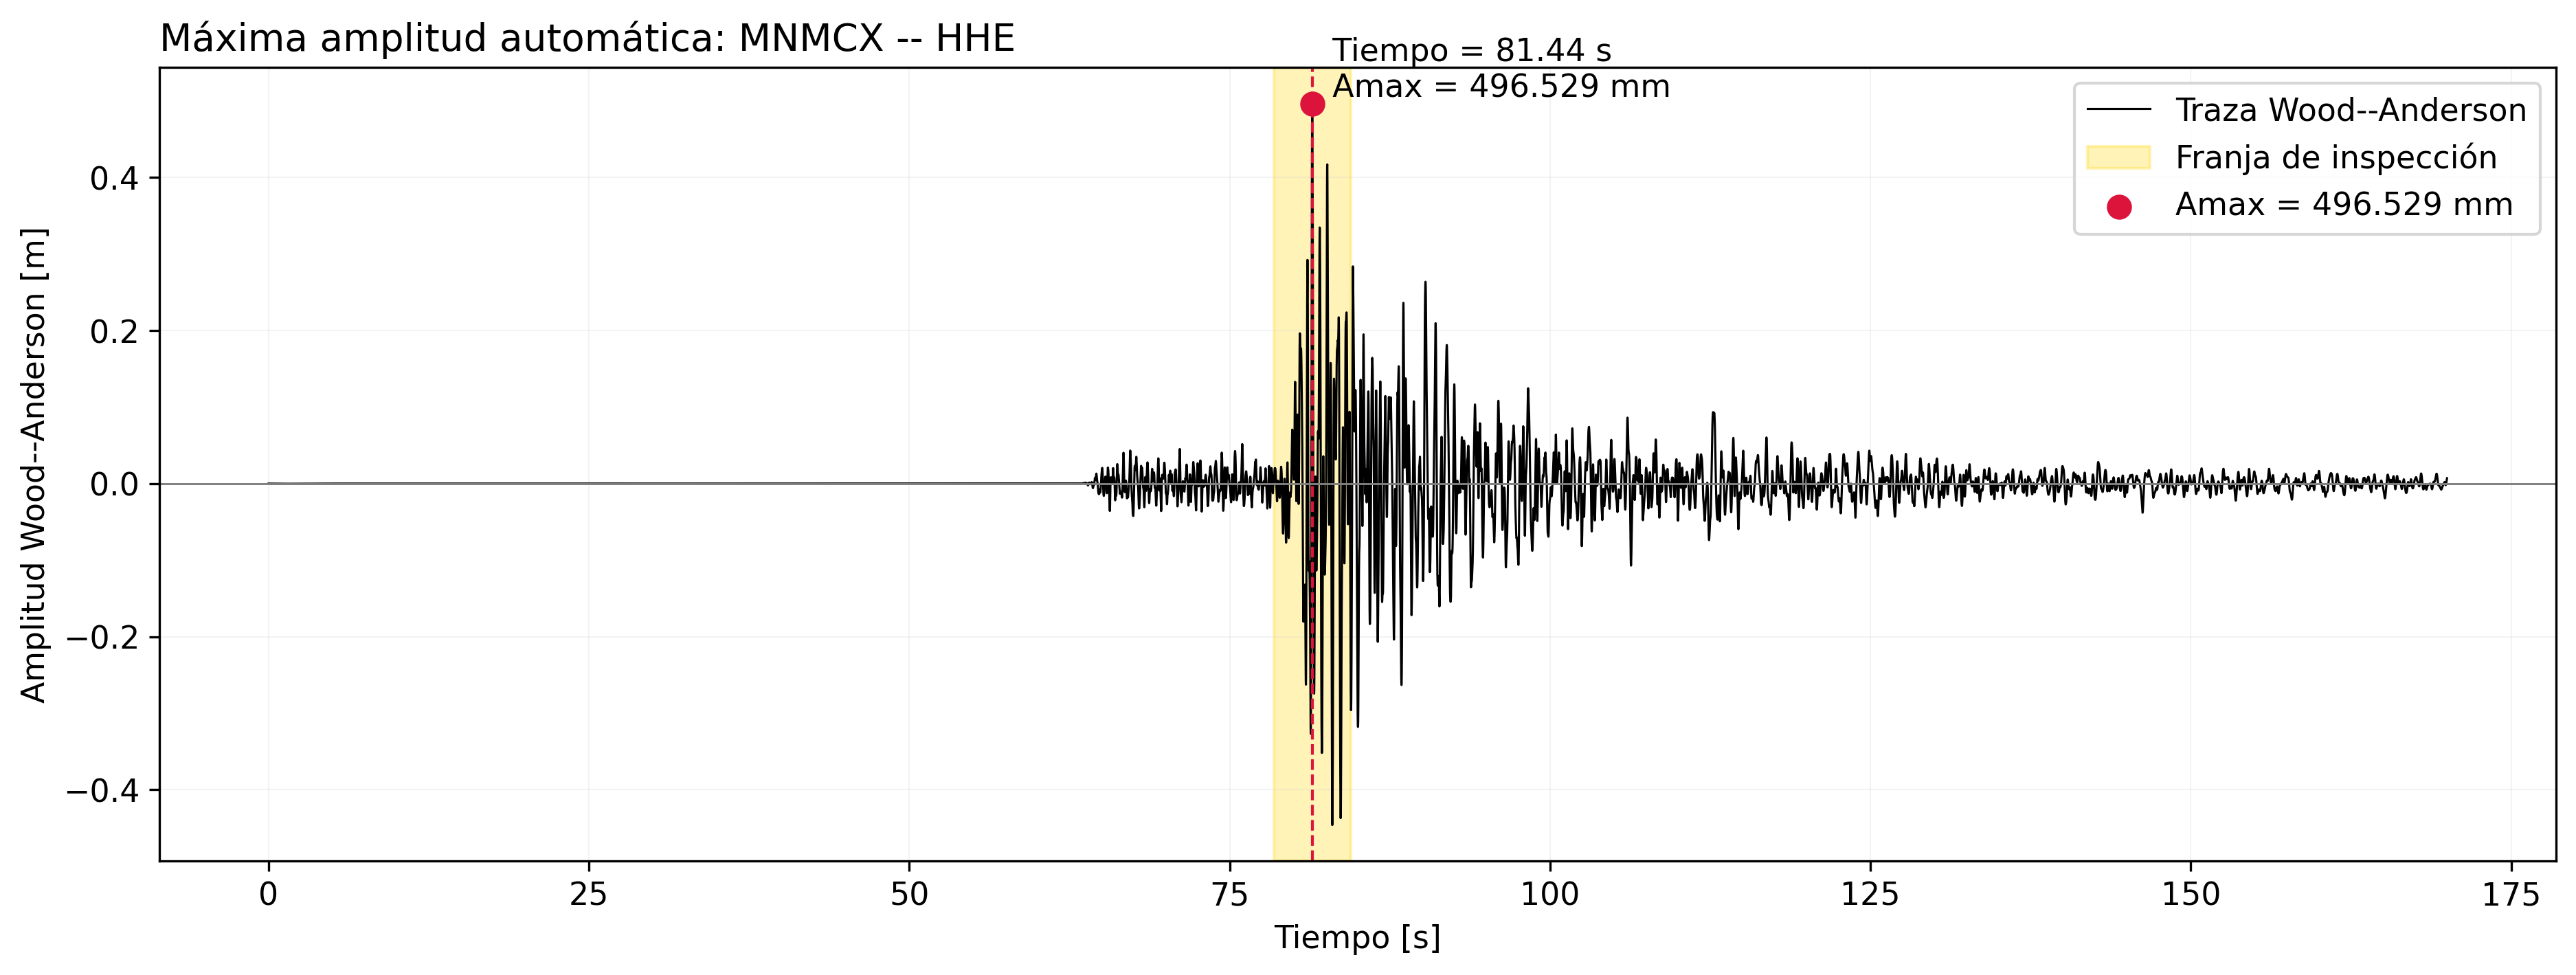
\includegraphics[width=0.95\textwidth]{Figures/amplitud_maxima_automatica}
    \caption{Ejemplo de detección automática de la amplitud máxima absoluta para la componente HHE de la estación MNMCX. La línea y el punto rojos indican la muestra de máxima amplitud, mientras que la franja amarilla representa la ventana visual de inspección alrededor de dicho máximo.}
    \label{fig:amplitud-maxima-automatica}
\end{figure}

El mismo procedimiento se repitió para las diez componentes horizontales disponibles. Los resultados de la detección automática se presentan en la Tabla~\ref{tab:amplitudes-maximas-wa}. La mayor amplitud máxima fue registrada por la componente HHE de la estación PATA, con \(622{,}355~\mathrm{mm}\), seguida por la componente HHN de la misma estación, con \(540{,}335~\mathrm{mm}\). En contraste, las menores amplitudes máximas se identificaron en las componentes de la estación PSGCX, con valores cercanos a \(140~\mathrm{mm}\).

\begin{table}[htbp]
    \centering
    \caption{Amplitudes máximas absolutas detectadas automáticamente en las componentes horizontales de los registros Wood--Anderson. La amplitud relativa corresponde al signo del desplazamiento en el instante de máximo valor absoluto.}
    \label{tab:amplitudes-maximas-wa}
    \begin{tabular}{l l r r r r}
        \hline
        Estación & Componente & Tiempo de $A_{\max}$ [s] &
        Amplitud rel [m] & $A_{\max}$ [m] & $A_{\max}$ [mm] \\
        \hline
        MNMCX & HHE & 81.44 &  0.496529 & 0.496529 & 496.529 \\
        MNMCX & HHN & 81.18 & -0.405633 & 0.405633 & 405.633 \\
        PATA  & HHE & 79.67 &  0.622355 & 0.622355 & 622.355 \\
        PATA  & HHN & 80.00 & -0.540335 & 0.540335 & 540.335 \\
        PB07  & HHE & 92.64 & -0.156229 & 0.156229 & 156.229 \\
        PB07  & HHN & 92.71 & -0.143698 & 0.143698 & 143.698 \\
        PSGCX & HHE & 79.33 & -0.140031 & 0.140031 & 140.031 \\
        PSGCX & HHN & 78.80 & -0.144421 & 0.144421 & 144.421 \\
        UNAP  & HHE & 75.24 &  0.288775 & 0.288775 & 288.775 \\
        UNAP  & HHN & 75.59 &  0.287222 & 0.287222 & 287.222 \\
        \hline
    \end{tabular}
\end{table}

\clearpage
Las amplitudes máximas fueron convertidas a milímetros e incorporadas en la relación de magnitud local junto con la distancia epicentral de cada estación, tal como se estableció en la sección de metodología. La Tabla~\ref{tab:ml-componentes-estaciones} presenta las magnitudes calculadas para las componentes E y N, así como la magnitud local promedio de cada estación. Las mayores estimaciones corresponden a PATA, con \(M_L=5{,}732\), y MNMCX, con \(M_L=5{,}708\). La menor magnitud promedio por estación se obtuvo para PSGCX, con \(M_L=5{,}156\).

\begin{table}[]
    \centering
    \caption{Resultados de magnitud local calculados por estación. Las columnas \(M_{L,E}\) y \(M_{L,N}\) corresponden a las componentes HHE y HHN, respectivamente.}
    \label{tab:ml-componentes-estaciones}
    \begin{tabular}{l r r r r}
        \hline
        Estación & $\Delta$ [km] & $M_{L,E}$ & $M_{L,N}$ &
        $M_{L,\mathrm{estación}}$ \\
        \hline
        MNMCX & 113.7 & 5.752 & 5.664 & 5.708 \\
        PATA  &  93.0 & 5.763 & 5.701 & 5.732 \\
        PB07  & 185.9 & 5.463 & 5.427 & 5.445 \\
        PSGCX & 100.7 & 5.149 & 5.163 & 5.156 \\
        UNAP  &  84.8 & 5.389 & 5.387 & 5.388 \\
        \hline
    \end{tabular}
\end{table}

A partir del promedio de las cinco magnitudes por estación se obtuvo una magnitud local final de:

\[
\overline{M_L} = 5{,}49.
\]

La desviación estándar entre estaciones fue de:

\[
\sigma_{M_L} = 0{,}24,
\]

mientras que el error estándar de la media fue:

\[
\mathrm{SEM}_{M_L} = 0{,}11.
\]

Por tanto, el mejor valor obtenido mediante esta metodología puede expresarse como:

\[
\boxed{
M_L = 5{,}49 \pm 0{,}24
}
\]

donde la incertidumbre indicada corresponde a la desviación estándar de las estimaciones entre estaciones. De manera alternativa, también se reporta la incertidumbre estadística asociada específicamente a la media, correspondiendo a:

\[
M_L = 5{,}49 \pm 0{,}11,
\]

utilizando el error estándar de la media en vez de la desviación estándar.

\vspace{1cm}
\fbox{%
    \begin{minipage}{\textwidth}
        El código empleado en el cálculo de la magnitud se encuentra en el adjunto \texttt{Calculo\_ML.pdf}. Este PDF muestra el notebook que carga automáticamente los archivos de las trazas Wood--Anderson, detecta las amplitudes máximas, calcula las magnitudes por componente y por estación, y finalmente obtiene la magnitud local promedio del evento junto con sus medidas de dispersión.
    \end{minipage}%
}

\clearpage
\subsection{Resultados de magnitud de momento \(M_w\)}

\subsubsection{Geometría fuente--estación}

Para la estimación del momento sísmico y de la magnitud de momento, se calculó inicialmente la distancia hipocentral entre el epicentro conocido del evento y cada estación. Aunque las distancias epicentrales describen la separación horizontal entre la proyección del evento y la estación, el cálculo de \(M_0\) requiere utilizar la distancia real entre la fuente sísmica y el receptor. Por esta razón, se empleó la relación:

\[
R =
\sqrt{\Delta^2+h^2},
\]

donde \(\Delta\) corresponde a la distancia epicentral y \(h=90~\mathrm{km}\) corresponde a la profundidad del evento. La distancia hipocentral se utilizó posteriormente en unidades de metros dentro de la ecuación de momento sísmico, dado que la amplitud espectral disminuye con la distancia de propagación.

\begin{table}[]
    \centering
    \caption{Distancias epicentrales e hipocentrales utilizadas para el cálculo de la magnitud de momento. La profundidad del evento corresponde a \(h=90~\mathrm{km}\).}
    \label{tab:distancias-hipocentrales}
    \begin{tabular}{l r r r}
        \hline
        Estación & Distancia epicentral $\Delta$ [km] &
        Profundidad $h$ [km] &
        Distancia hipocentral $R$ [km] \\
        \hline
        MNMCX & 113.7 & 90.0 & 145.01 \\
        PATA  &  93.0 & 90.0 & 129.42 \\
        PB07  & 185.9 & 90.0 & 206.54 \\
        PSGCX & 100.7 & 90.0 & 135.06 \\
        UNAP  &  84.8 & 90.0 & 123.66 \\
        \hline
    \end{tabular}
\end{table}

La Tabla~\ref{tab:distancias-hipocentrales} presenta las distancias epicentrales entregadas para cada estación y las distancias hipocentrales calculadas. La estación PB07 presenta la mayor distancia hipocentral, con \(206{,}54~\mathrm{km}\), mientras que UNAP presenta la menor distancia hipocentral, con \(123{,}66~\mathrm{km}\).


\subsubsection{Registros de desplazamiento y selección de ventanas S}

Para el análisis espectral se utilizaron los registros de desplazamiento de las estaciones MNMCX, PATA, PB07, PSGCX y UNAP. Cada estación cuenta con tres componentes: este--oeste (\texttt{HHE}), norte--sur (\texttt{HHN}) y vertical (\texttt{HHZ}). En total se analizaron 15 trazas de desplazamiento, cada una de ellas contiene 17001 muestras, posee una duración de 170~s y fueron registradas con una frecuencia de muestreo de \(100~\mathrm{Hz}\).

La Figura~\ref{fig:registros-desplazamiento} presenta los registros de desplazamiento de las tres componentes para cada estación. En las trazas se observa una llegada inicial de menor amplitud, asociada a la onda P, seguida por un incremento más pronunciado de la amplitud que corresponde a la llegada de la onda S y su coda temprana. La separación temporal entre ambas fases cambia entre estaciones debido a las diferencias en la distancia hipocentral y en la geometría de propagación fuente--estación. En particular, las estaciones más alejadas, como PB07, presentan una separación temporal más amplia entre los principales paquetes de energía, mientras que las estaciones con menor distancia hipocentral, como UNAP y PATA, muestran arribos más cercanos en el tiempo.

\begin{figure}[htbp]
    \centering
    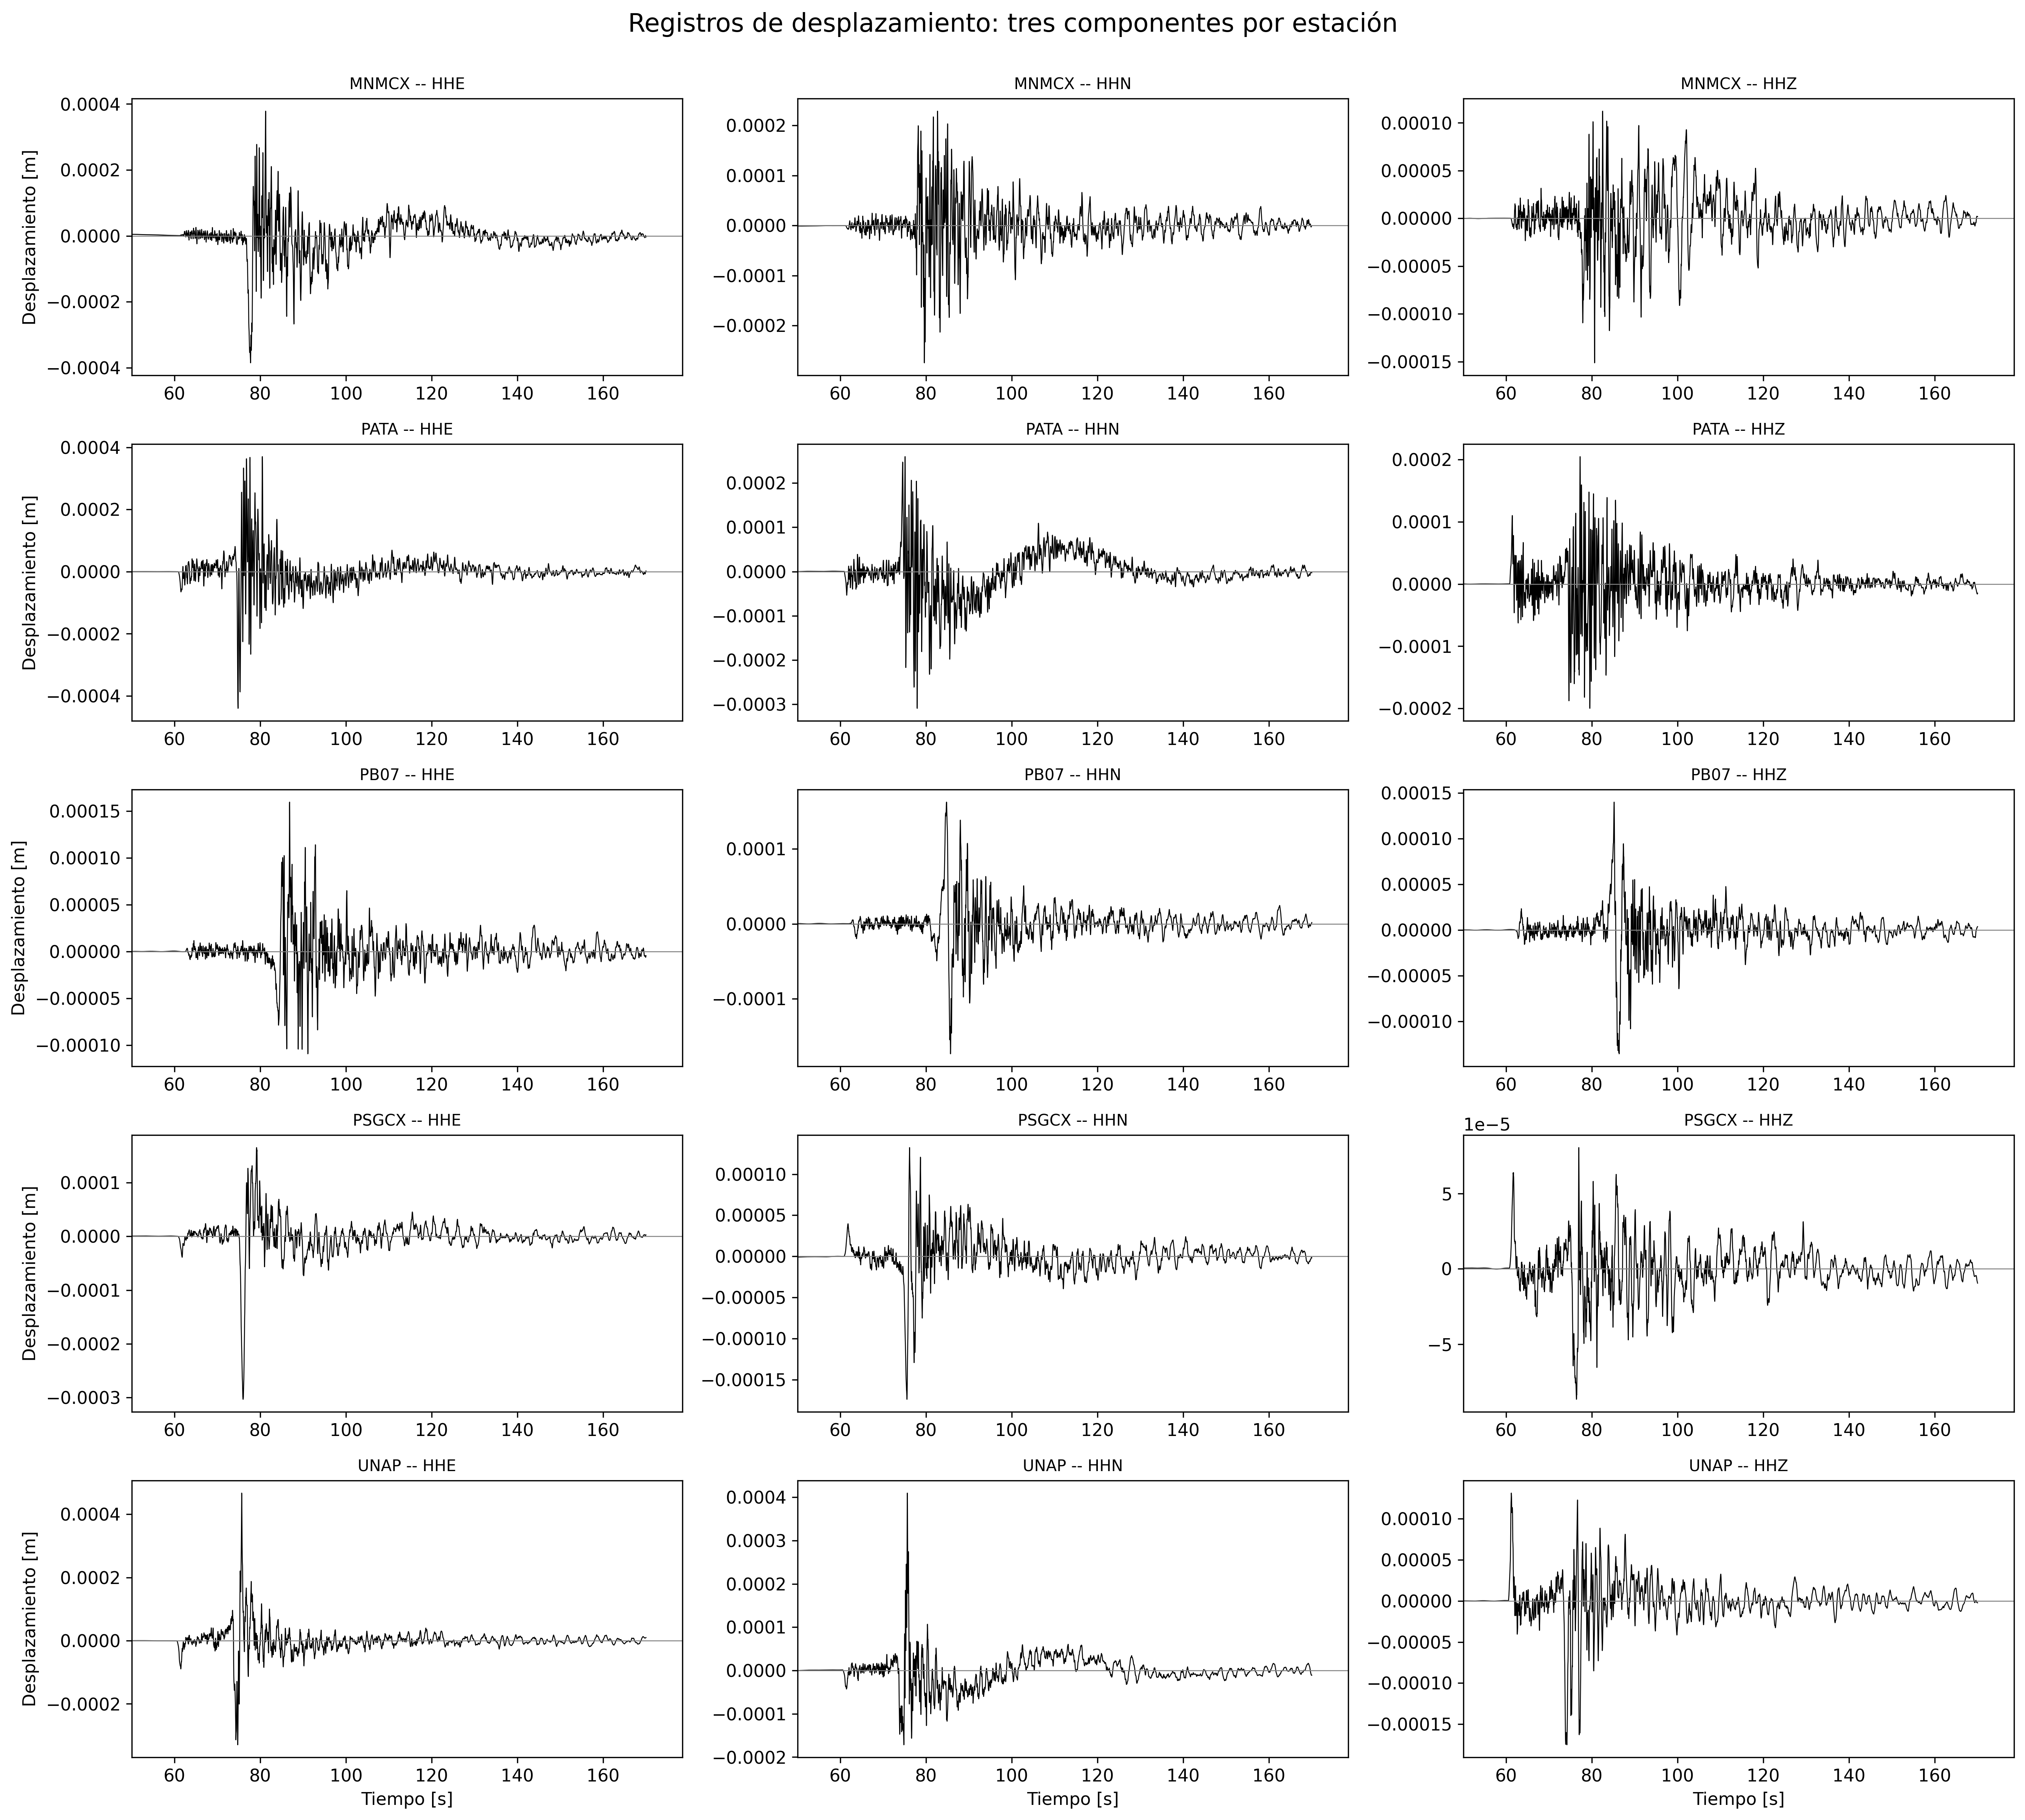
\includegraphics[width=\textwidth]{Figures/Registros_desplazamiento_tres_componentes.png}
    \caption{Registros de desplazamiento de las tres componentes para las estaciones MNMCX, PATA, PB07, PSGCX y UNAP. Las trazas se utilizaron para identificar visualmente la llegada de la onda S y seleccionar las ventanas temporales empleadas en el análisis espectral.}
    \label{fig:registros-desplazamiento}
\end{figure}

La selección de las ventanas de onda S se realizó mediante inspección visual individual de las tres componentes de cada estación. Se eligieron intervalos que incluyeran la fase S y una parte de su coda temprana, procurando excluir la fase P y los segmentos tardíos dominados por ruido. La duración de cada ventana determina la resolución espectral mínima:

\[
\delta f =
\frac{1}{t_{\mathrm{fin}}-t_{\mathrm{ini}}}.
\]
Esta frecuencia fué usada como valor preliminar de la banda de frecuencias para el ajuste de la plateau en el espectro de Fourier. Posteriormente, para cada ventana se calculó el espectro de amplitud de desplazamiento y se seleccionó visualmente una banda de baja frecuencia para estimar el plateau espectral, actualizando el valor preliminarmente usado antes. La selección se realizó considerando la región de comportamiento más estable de las tres componentes, evitando el valor de frecuencia cero, los primeros bins de frecuencia potencialmente afectados por tendencia residual o duración finita de la ventana, los picos estrechos y el tramo de mayor frecuencia donde comienza el decaimiento espectral.

\begin{figure}[]
    \centering

    \begin{subfigure}[b]{0.49\textwidth}
        \centering
        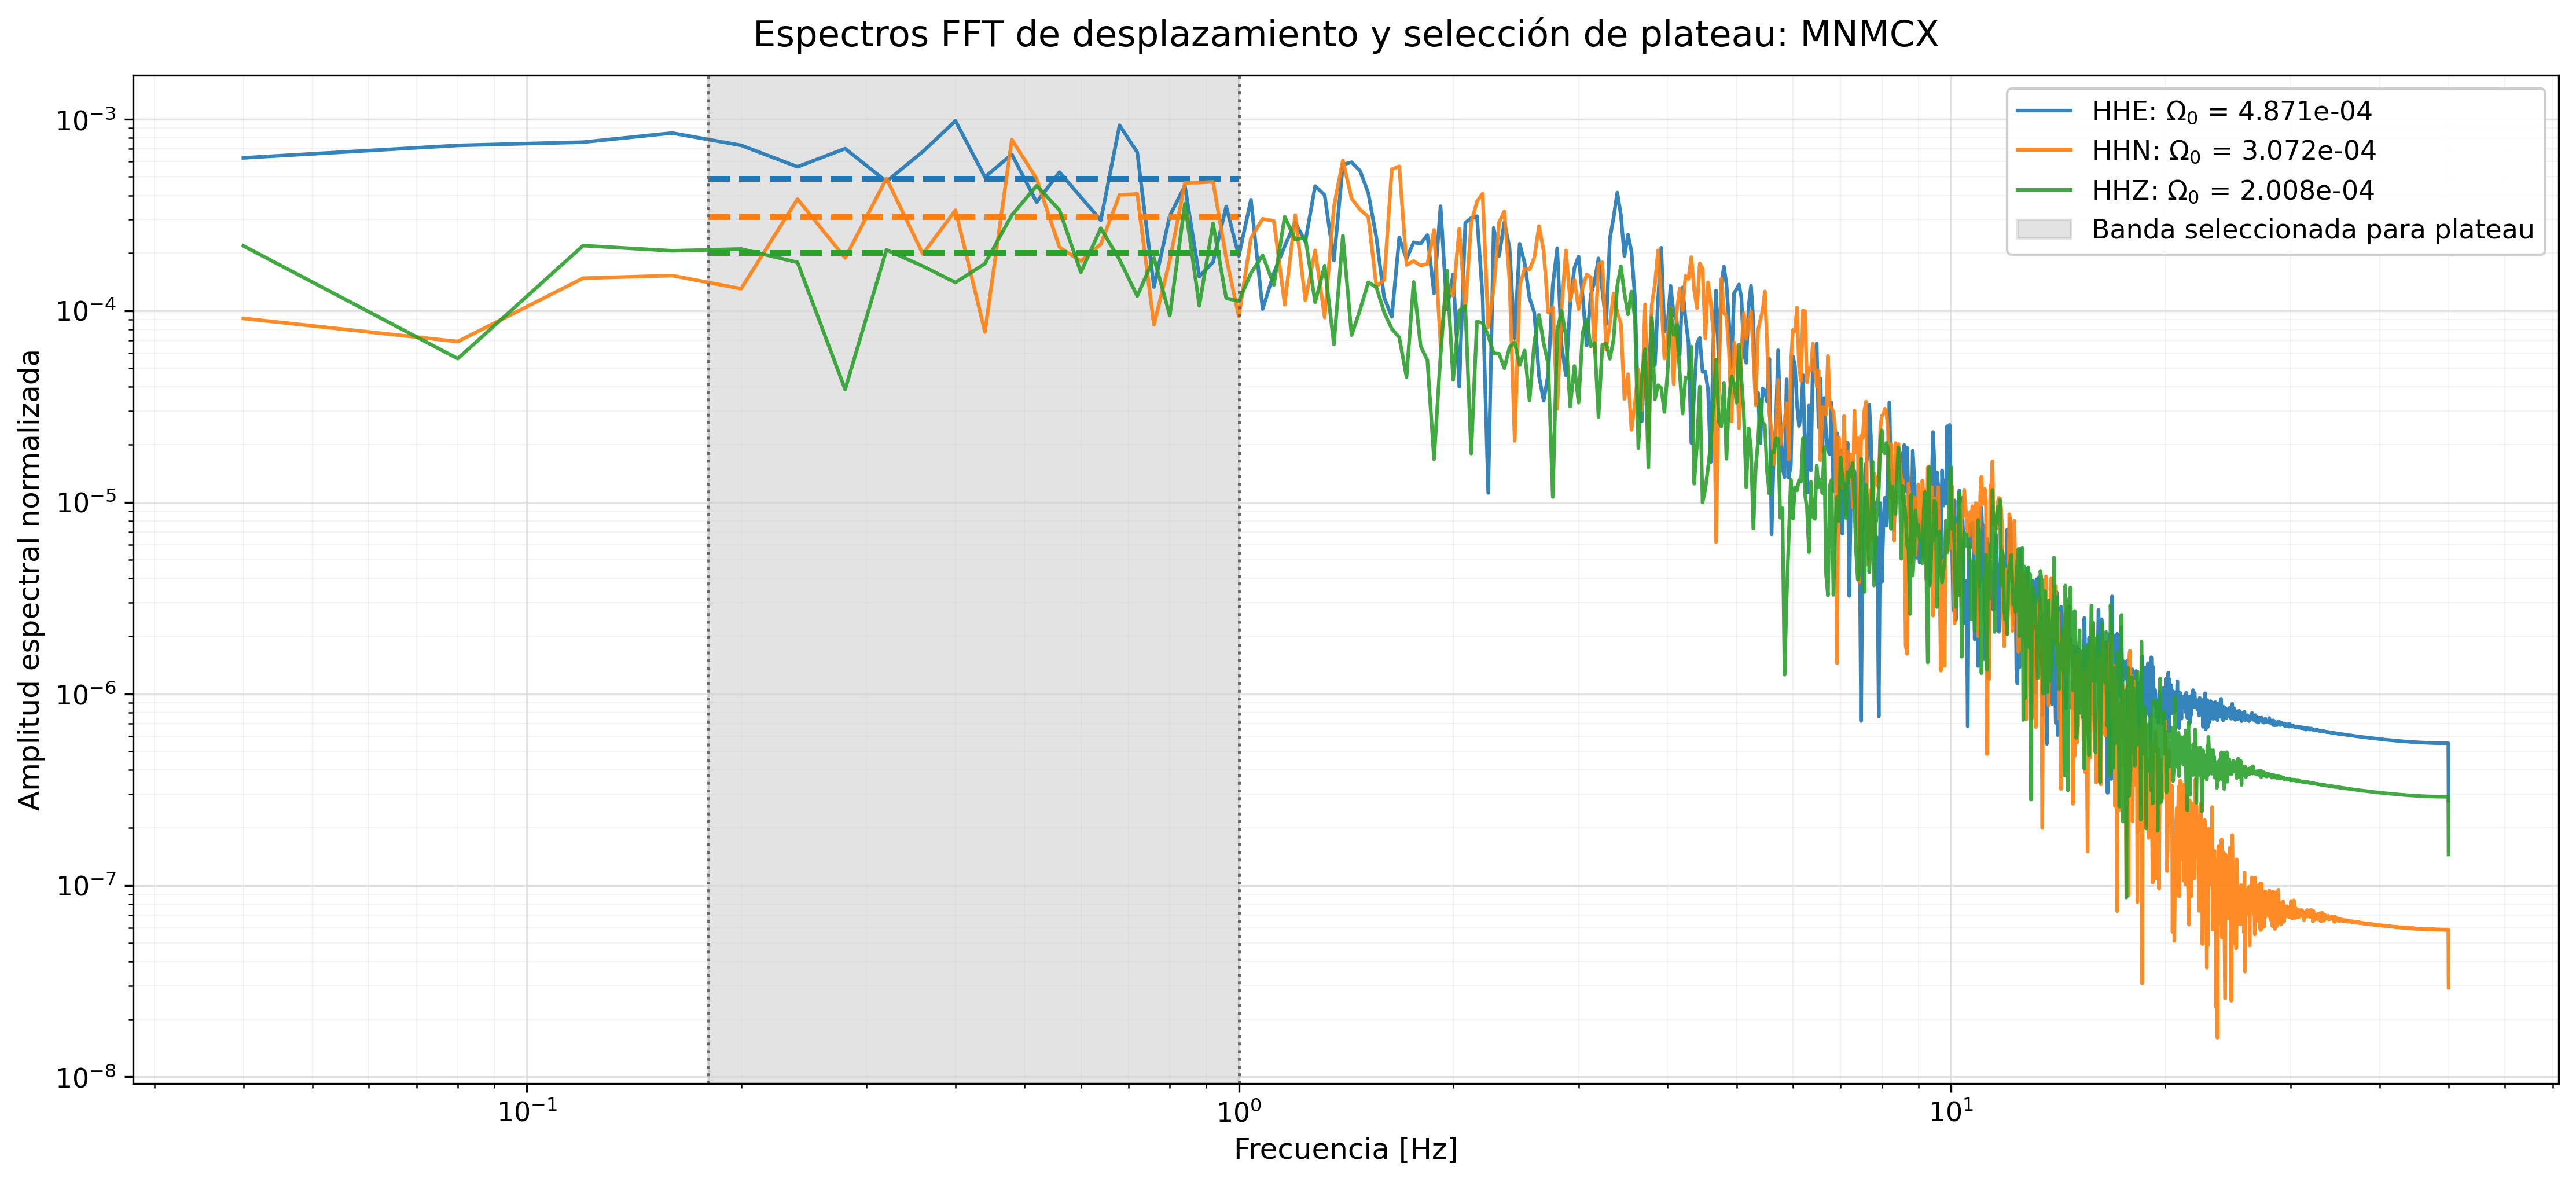
\includegraphics[width=\textwidth]{Figures/FFT_plateau_MNMCX.png}
        \caption{Estación MNMCX.}
        \label{fig:fft-mnmcx}
    \end{subfigure}
    \hfill
    \begin{subfigure}[b]{0.49\textwidth}
        \centering
        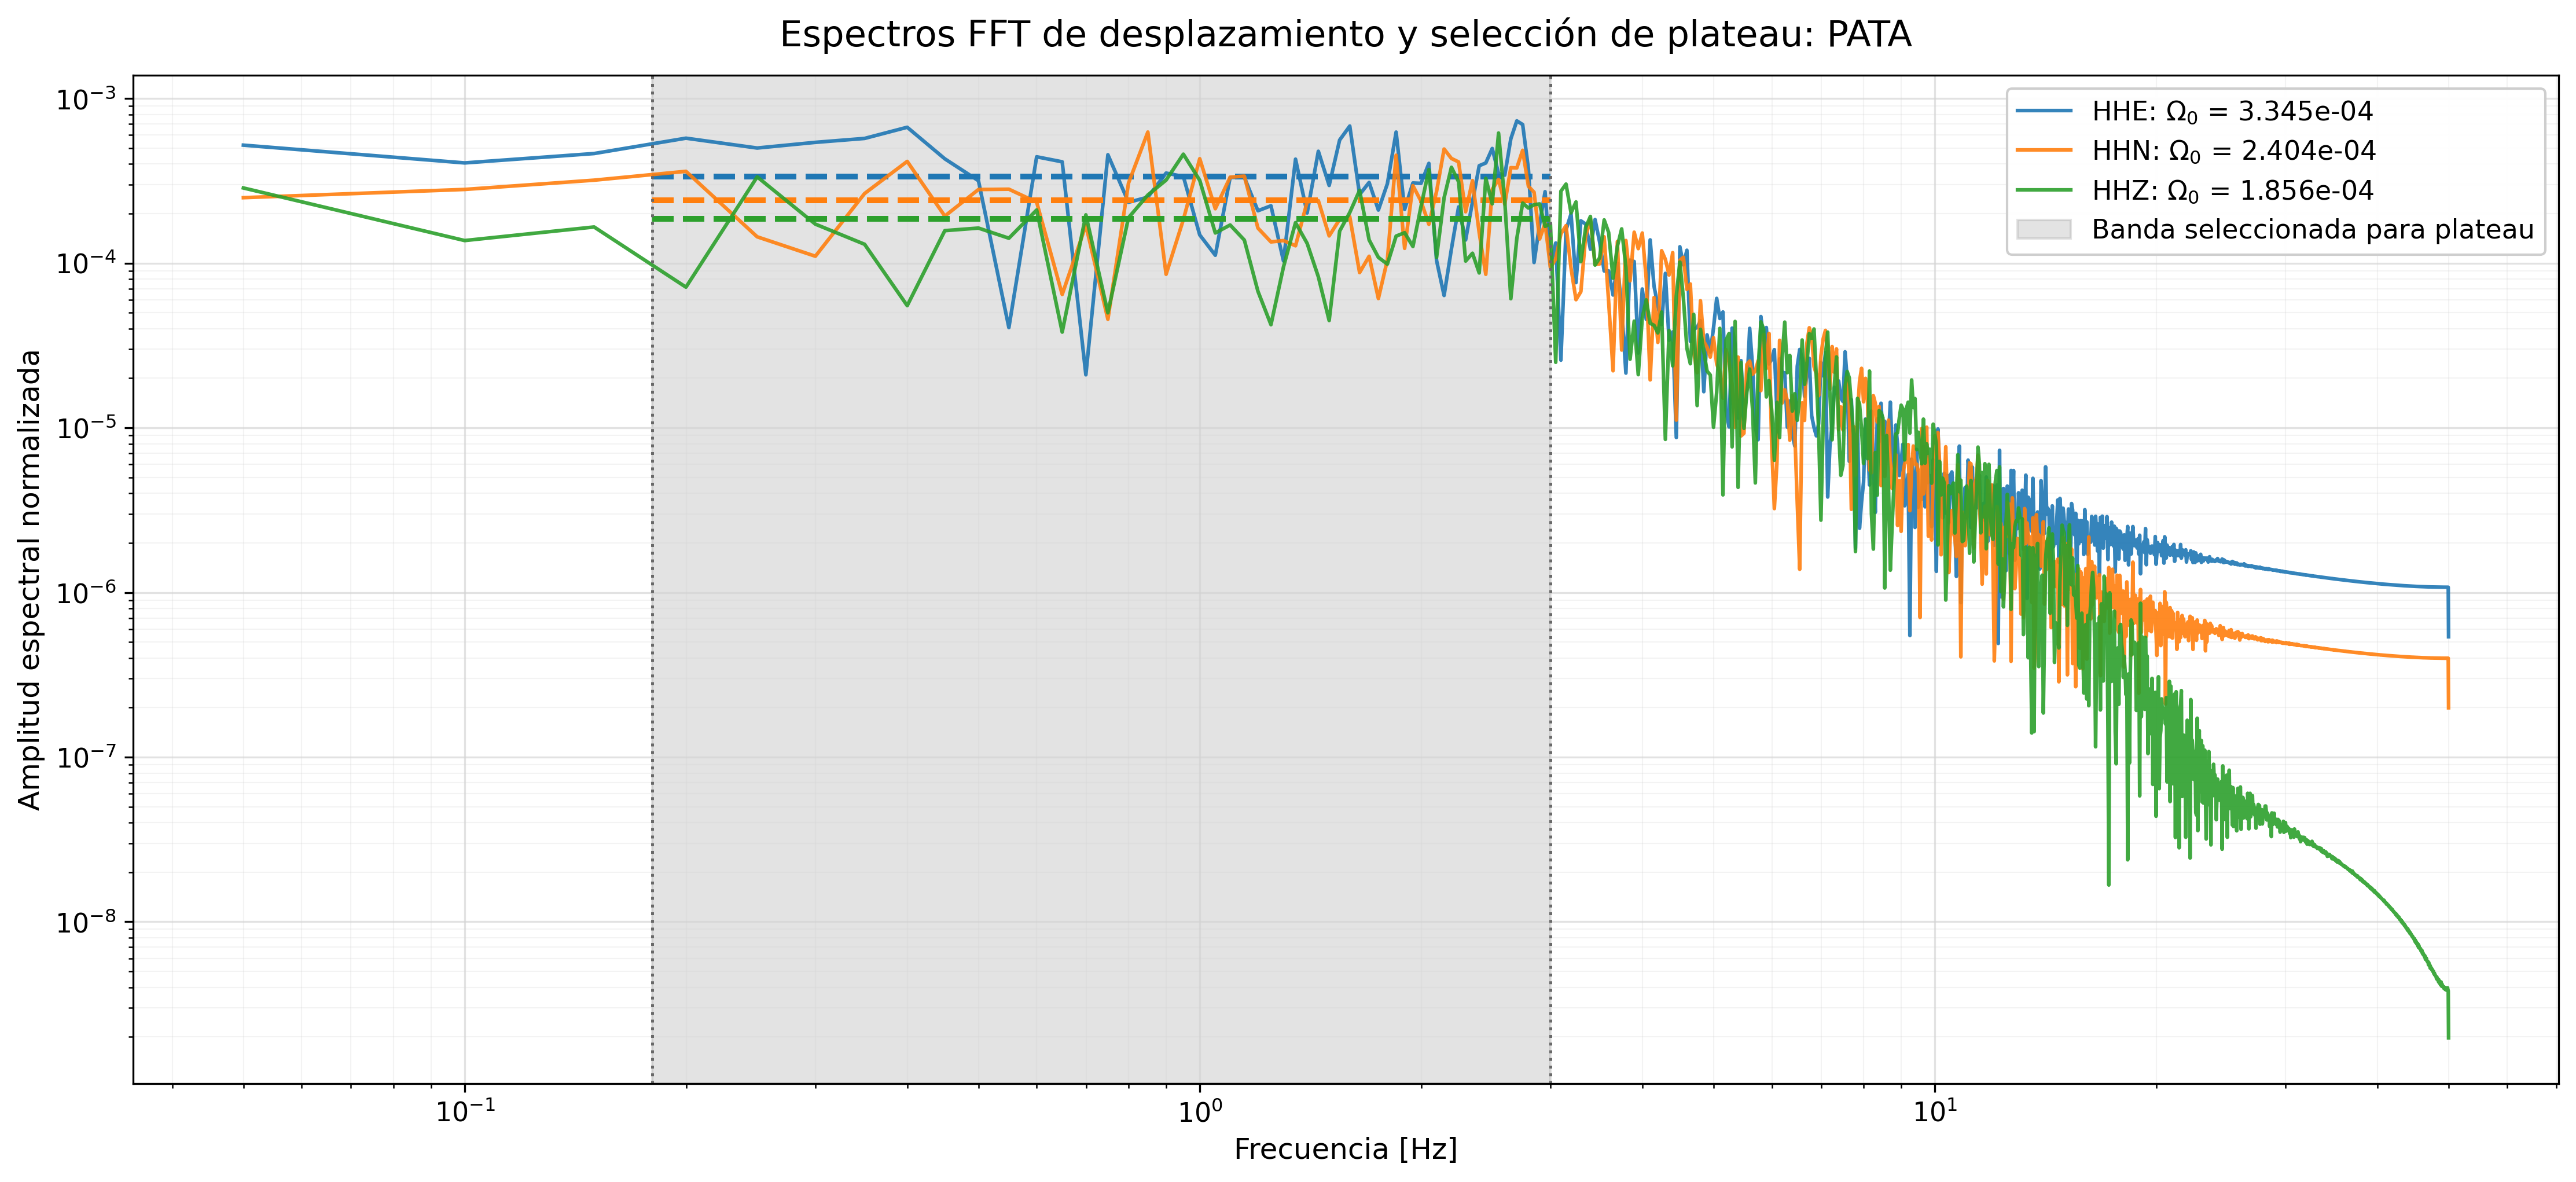
\includegraphics[width=\textwidth]{Figures/FFT_plateau_PATA.png}
        \caption{Estación PATA.}
        \label{fig:fft-pata}
    \end{subfigure}

    \vspace{0.5cm}

    \begin{subfigure}[b]{0.49\textwidth}
        \centering
        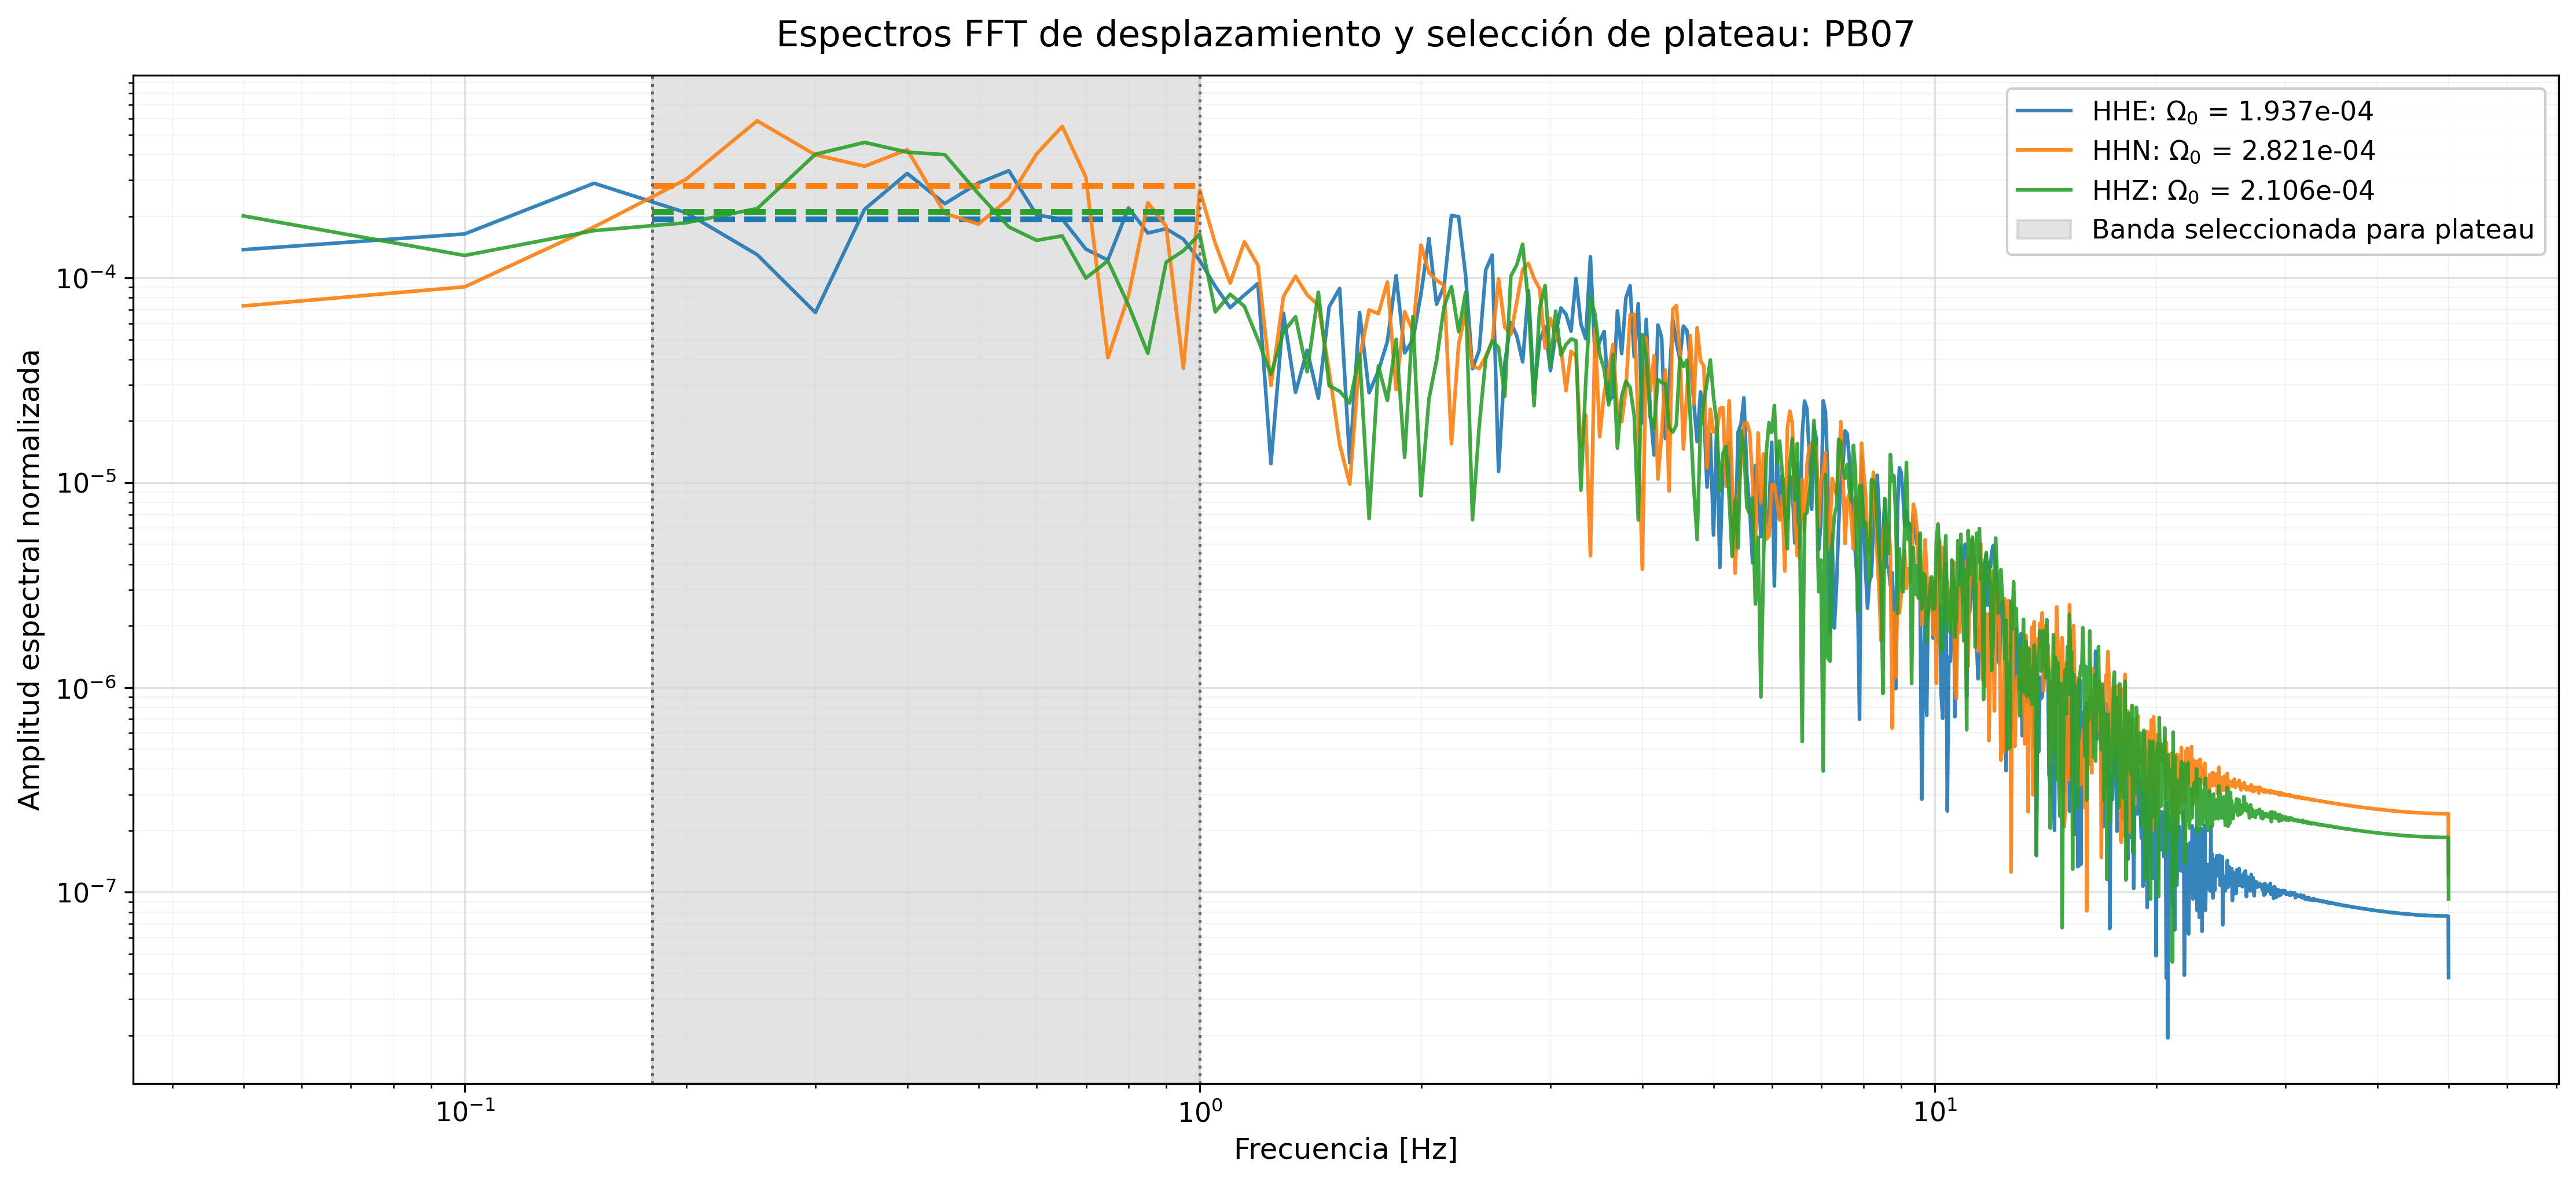
\includegraphics[width=\textwidth]{Figures/FFT_plateau_PB07.png}
        \caption{Estación PB07.}
        \label{fig:fft-pb07}
    \end{subfigure}
    \hfill
    \begin{subfigure}[b]{0.49\textwidth}
        \centering
        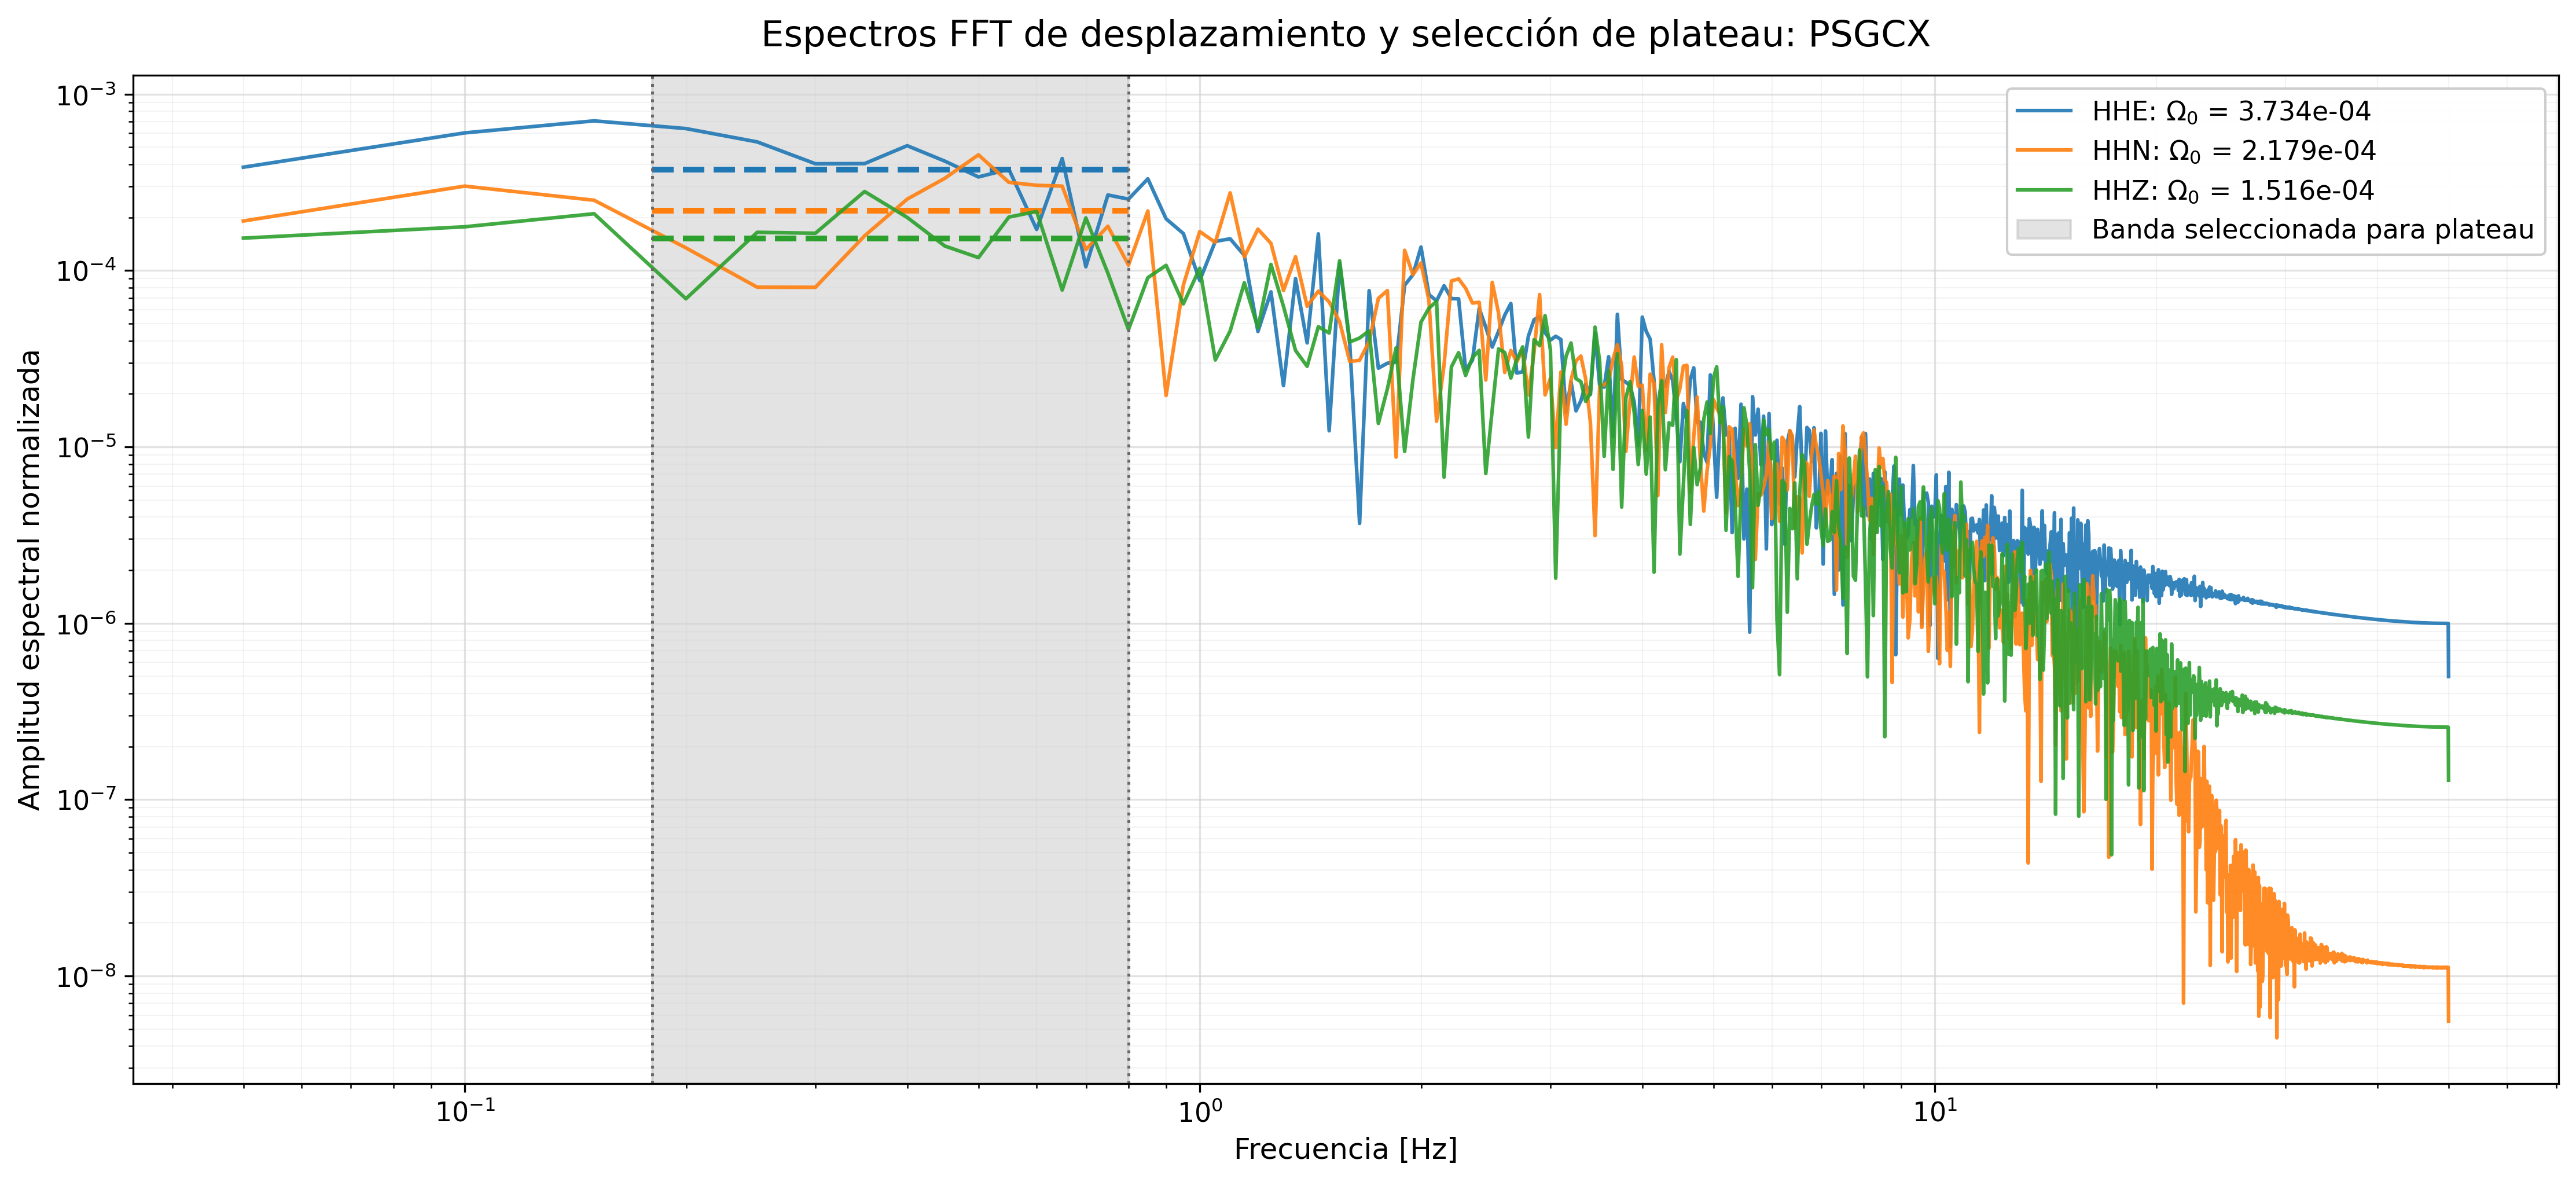
\includegraphics[width=\textwidth]{Figures/FFT_plateau_PSGCX.png}
        \caption{Estación PSGCX.}
        \label{fig:fft-psgcx}
    \end{subfigure}

    \vspace{0.5cm}

    \begin{subfigure}[b]{0.61\textwidth}
        \centering
        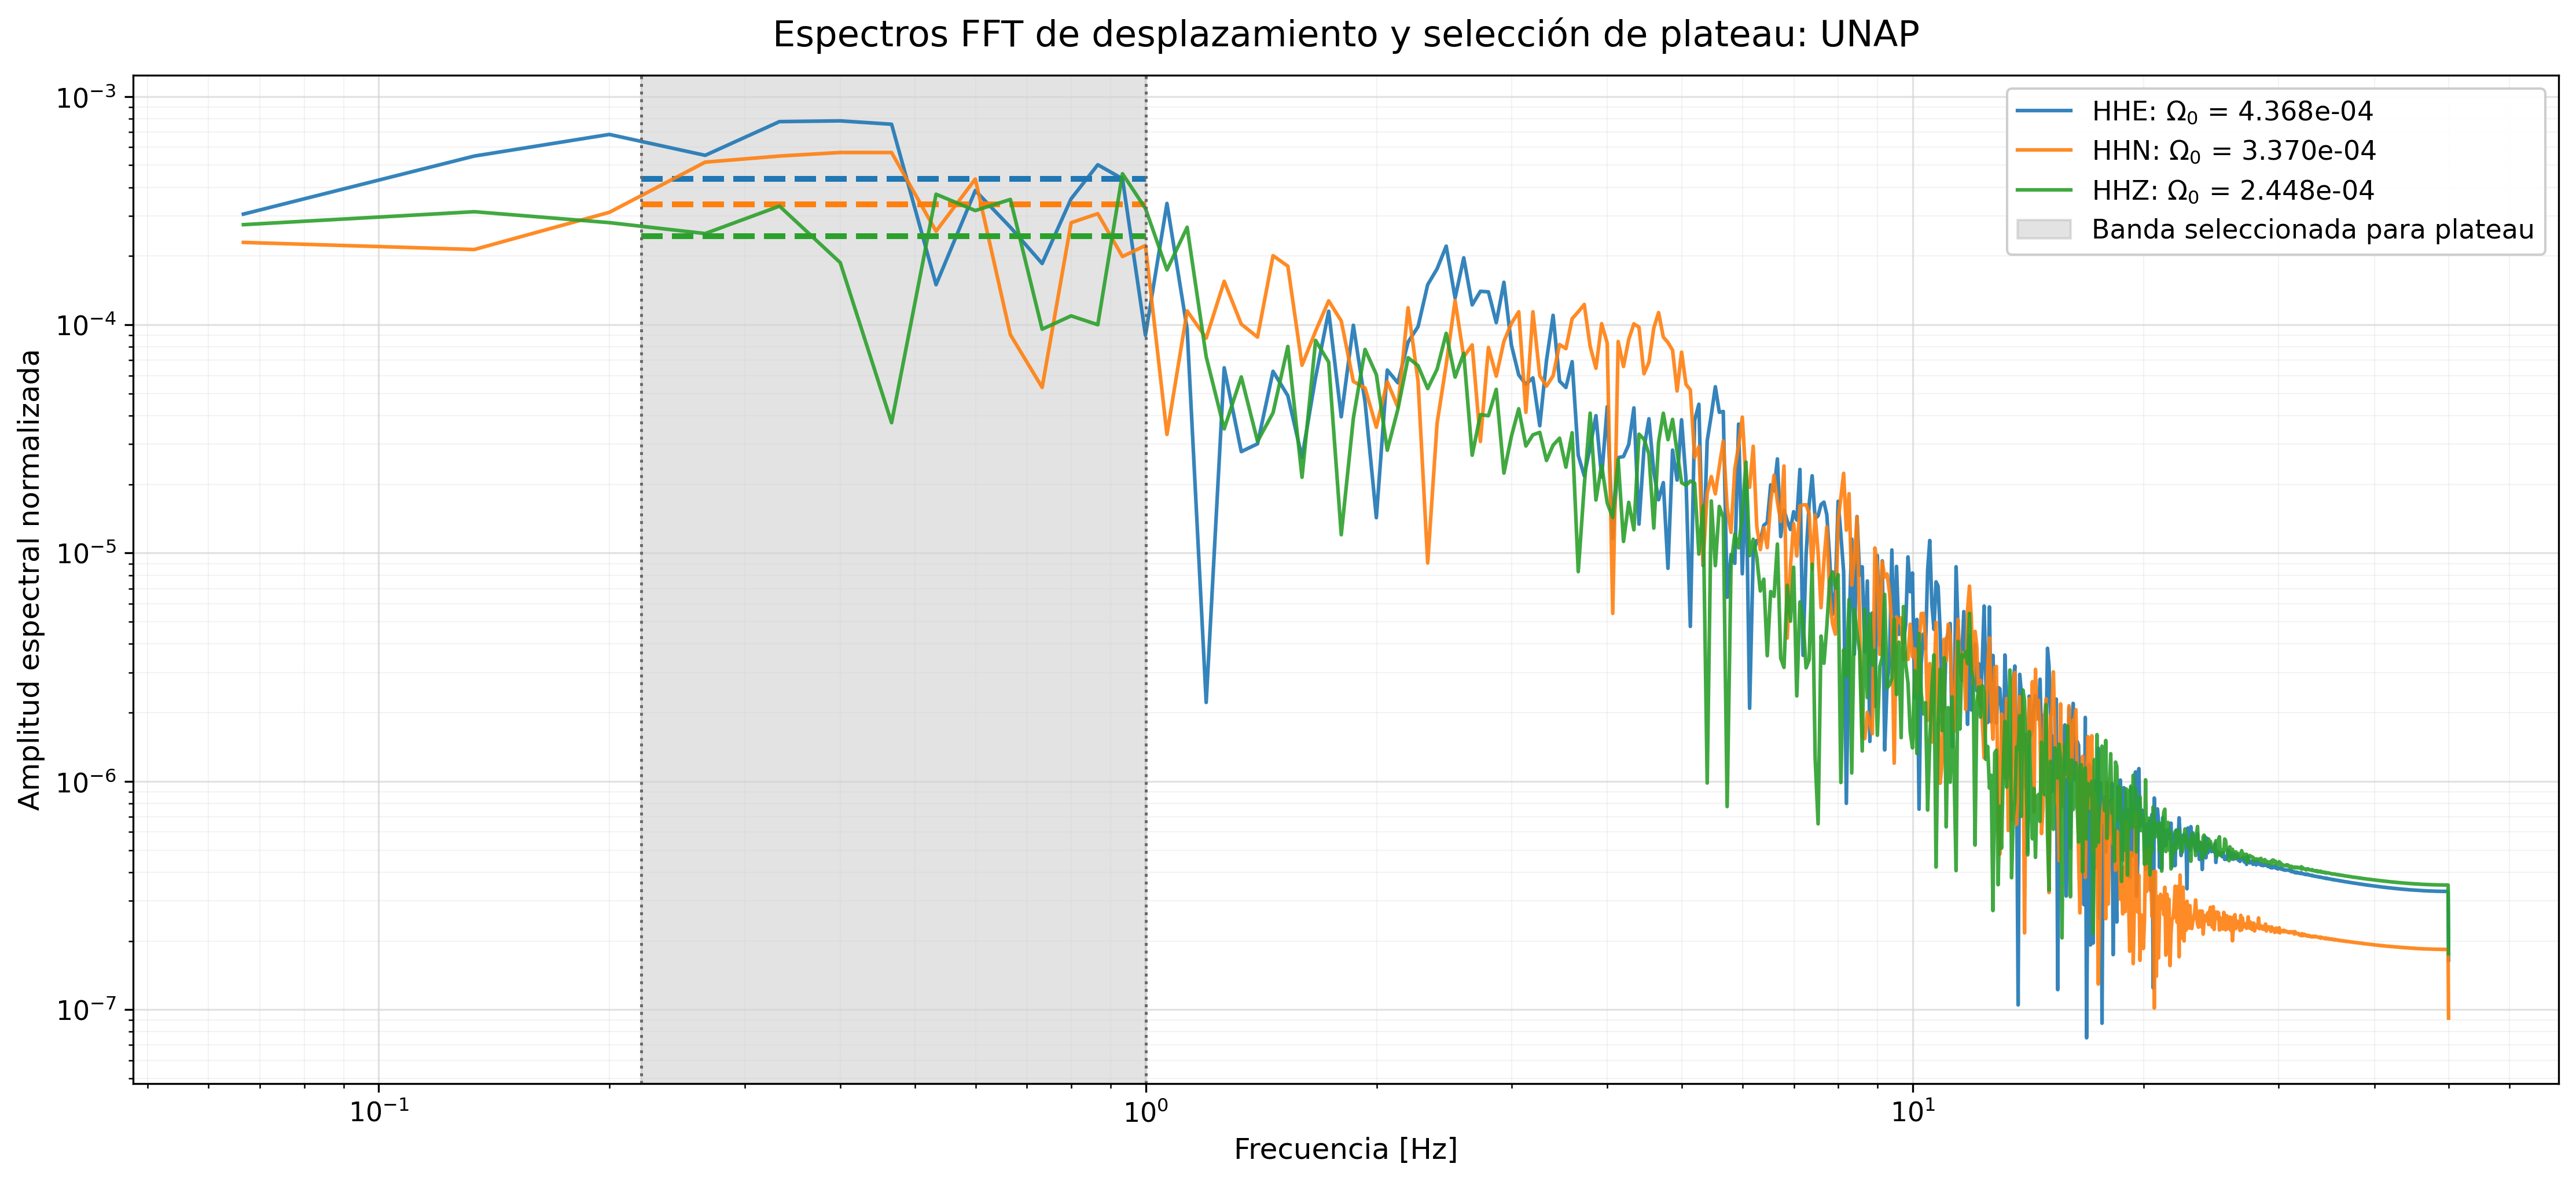
\includegraphics[width=\textwidth]{Figures/FFT_plateau_UNAP.png}
        \caption{Estación UNAP.}
        \label{fig:fft-unap}
    \end{subfigure}

    \caption{Espectros FFT de desplazamiento obtenidos para las cinco estaciones. Las curvas azul, naranja y verde representan las componentes HHE, HHN y HHZ, respectivamente. Las bandas grises indican los intervalos de frecuencia empleados para estimar los plateaus espectrales.}
    \label{fig:espectros-plateau}
\end{figure}

Los resultados obtenidos de la selección de frecuencias se resumen en la Figura~\ref{fig:espectros-plateau}. Esta figura reúne los espectros FFT obtenidos para las cinco estaciones, en cada panel se muestran los espectros de las componentes HHE, HHN y HHZ, junto con la banda sombreada utilizada para el cálculo del plateau. La banda seleccionada corresponde al intervalo en el que se promedió la amplitud espectral para obtener \(\Omega_E\), \(\Omega_N\) y \(\Omega_Z\).

\clearpage

En ese sentido, la Tabla~\ref{tab:ventanas-plateaus} resume las ventanas temporales seleccionadas para la onda S y las bandas de frecuencia empleadas en la estimación de los plateaus. Las ventanas utilizadas tuvieron duraciones entre 15 y 25~s, lo que se traduce en distintas resoluciones espectrales. La estación UNAP utilizó la ventana más corta, desde 70 hasta 85~s, mientras que MNMCX utilizó una ventana de 25~s, que va desde los 75 hasta los 100~s.

\begin{table}[]
    \centering
    \caption{Ventanas de onda S y bandas de frecuencia seleccionadas para el cálculo del plateau espectral en cada estación.}
    \label{tab:ventanas-plateaus}
    \begin{tabular}{l r r r r r r}
        \hline
        Estación &
        Inicio S [s] &
        Final S [s] &
        $f_{\min}$ [Hz] &
        $f_{\max}$ [Hz] &
        $f_s$ [Hz] &
        Muestras \\
        \hline
        MNMCX & 75.0 & 100.0 & 0.18 & 1.00 & 100.0 & 2501 \\
        PATA  & 70.0 &  90.0 & 0.18 & 3.00 & 100.0 & 2001 \\
        PB07  & 80.0 & 100.0 & 0.18 & 1.00 & 100.0 & 2001 \\
        PSGCX & 70.0 &  90.0 & 0.18 & 0.80 & 100.0 & 2001 \\
        UNAP  & 70.0 &  85.0 & 0.22 & 1.00 & 100.0 & 1501 \\
        \hline
    \end{tabular}
\end{table}

En cada espectro se ajustó una línea horizontal discontinua sobre la banda de frecuencia seleccionada (véase la Figura \ref{fig:espectros-plateau}). Esta línea corresponde al promedio aritmético de las amplitudes espectrales dentro del intervalo elegido y representa la estimación del plateau para cada una de las componentes. Es decir, se obtuvieron los parámetros:

\[\Omega_E,\qquad \Omega_N, \qquad \Omega_Z\]

para cada estación, los cuales se combinaron posteriormente para calcular la magnitud de momento.

El cálculo del plateau se efectuó después de remover la tendencia lineal de la ventana S y de normalizar la transformada rápida de Fourier por el número de muestras de la ventana. Para representar un espectro unilateral de amplitud, las amplitudes de las frecuencias internas fueron duplicadas, excluyendo la frecuencia cero. La frecuencia cero fue excluida porque representa la componente DC del registro y puede estar afectada por tendencias residuales. También se evitaron las frecuencias extremadamente bajas, donde la resolución limitada por la duración de la ventana puede producir estimaciones inestables. Por otra parte, no se incluyeron las frecuencias donde las curvas muestran picos aislados, oscilaciones intensas o un decaimiento sistemático de la amplitud, ya que estas regiones no representan de manera adecuada el nivel de baja frecuencia asociado al momento sísmico. La estimación de las rectas horizontales se restringió a las bandas de baja frecuencia indicadas en la Figura~\ref{fig:espectros-plateau}.

\subsubsection{Plateaus espectrales, momento sísmico y magnitud de momento}

A partir de las ventanas de onda S y de las bandas de frecuencia seleccionadas para cada estación, se estimaron los plateaus espectrales de las tres componentes de desplazamiento. Los valores obtenidos corresponden a los niveles promedio de amplitud espectral dentro de la banda de baja frecuencia seleccionada para cada componente: \(\Omega_E\) para la componente este--oeste, \(\Omega_N\) para la componente norte--sur y \(\Omega_Z\) para la componente vertical.

La Tabla~\ref{tab:plateaus-componentes} presenta los plateaus obtenidos para las cinco estaciones. Los valores se encuentran en el mismo orden de magnitud, entre aproximadamente \(1{,}52\times10^{-4}\) y \(4{,}87\times10^{-4}\), aunque se observa variabilidad entre componentes y estaciones. En particular, MNMCX presenta el mayor plateau para la componente este--oeste, mientras que PSGCX presenta el valor más bajo para la componente vertical. Estas diferencias reflejan variaciones en la amplitud registrada, la geometría fuente--estación, la orientación de las componentes y la respuesta local de cada sitio.

\clearpage

\begin{table}[]
    \centering
    \caption{Plateaus espectrales de desplazamiento obtenidos para las tres componentes de cada estación. Los valores corresponden al promedio de la amplitud espectral dentro de la banda de baja frecuencia seleccionada.}
    \label{tab:plateaus-componentes}
    \begin{tabular}{l r r r}
        \hline
        Estación & $\Omega_E$ & $\Omega_N$ & $\Omega_Z$ \\
        \hline
        MNMCX & $4.871219\times10^{-4}$ & $3.072301\times10^{-4}$ & $2.008495\times10^{-4}$ \\
        PATA  & $3.345003\times10^{-4}$ & $2.403759\times10^{-4}$ & $1.856234\times10^{-4}$ \\
        PB07  & $1.937365\times10^{-4}$ & $2.820680\times10^{-4}$ & $2.105542\times10^{-4}$ \\
        PSGCX & $3.734107\times10^{-4}$ & $2.178766\times10^{-4}$ & $1.515588\times10^{-4}$ \\
        UNAP  & $4.367691\times10^{-4}$ & $3.370381\times10^{-4}$ & $2.447575\times10^{-4}$ \\
        \hline
    \end{tabular}
\end{table}

Para reducir la dependencia de una componente individual, los tres plateaus de cada estación se combinaron mediante una media cuadrática:

\[
\Omega_{\mathrm{RMS}} =
\left(
\frac{
\Omega_E^2+\Omega_N^2+\Omega_Z^2
}{3}
\right)^{1/2}.
\]

Este valor representa una amplitud espectral combinada para la estación e incorpora la información de las componentes horizontales y vertical. Posteriormente, \(\Omega_{\mathrm{RMS}}\) se utilizó junto con la distancia hipocentral, la densidad, la velocidad de onda S, el factor de superficie libre y el patrón de radiación promedio para calcular el momento sísmico:

\[
M_0 =  \frac{4\pi\rho\beta^3R}{ V\langle R_S \rangle } \Omega_{\mathrm{RMS}}.
\]

Finalmente, el momento sísmico de cada estación fue convertido a magnitud de momento mediante:

\[
M_w =
\frac{2}{3}\log_{10}(M_0)-6{,}07.
\]

La Tabla~\ref{tab:momento-mw-estaciones} presenta los resultados obtenidos por estación. Los momentos sísmicos calculados se encuentran entre \(1{,}17\times10^{17}~\mathrm{N\,m}\) y \(1{,}77\times10^{17}~\mathrm{N\,m}\), mientras que las magnitudes de momento individuales varían entre \(M_w=5{,}308\) y \(M_w=5{,}428\). La estación MNMCX presenta la mayor estimación de momento sísmico y de magnitud de momento, mientras que PATA presenta el menor valor de \(M_w\).

\begin{table}[]
    \centering
    \caption{Resultados del cálculo de momento sísmico y magnitud de momento por estación. \(\Omega_{\mathrm{RMS}}\) corresponde a la combinación cuadrática de los plateaus de las tres componentes.}
    \label{tab:momento-mw-estaciones}
    \begin{tabular}{l r r r r}
        \hline
        Estación & $R$ [km] & $\Omega_{\mathrm{RMS}}$ &
        $M_0$ [N\,m] & $M_w$ \\
        \hline
        MNMCX & 145.01 & $3.521451\times10^{-4}$ & $1.767758\times10^{17}$ & 5.428 \\
        PATA  & 129.42 & $2.608493\times10^{-4}$ & $1.168664\times10^{17}$ & 5.308 \\
        PB07  & 206.54 & $2.319693\times10^{-4}$ & $1.658595\times10^{17}$ & 5.410 \\
        PSGCX & 135.06 & $2.644969\times10^{-4}$ & $1.236643\times10^{17}$ & 5.325 \\
        UNAP  & 123.66 & $3.484576\times10^{-4}$ & $1.491674\times10^{17}$ & 5.379 \\
        \hline
    \end{tabular}
\end{table}

La magnitud de momento final se obtuvo promediando las cinco estimaciones individuales:

\[
\overline{M_w} =
\frac{1}{5}
\sum_{i=1}^{5}M_{w,i}.
\]

El valor promedio obtenido fue:

\[
\overline{M_w} = 5{,}370.
\]

La mediana de las estimaciones fue \(5{,}379\), la desviación estándar entre estaciones fue \(0{,}052\) y el error estándar de la media fue \(0{,}023\). Por tanto, el resultado final puede expresarse como:

\[
\boxed{
M_w = 5{,}37 \pm 0{,}05
}
\]

donde la incertidumbre corresponde a la desviación estándar de las estimaciones obtenidas en las cinco estaciones. Si se desea expresar exclusivamente la incertidumbre estadística asociada al valor promedio, el resultado puede reportarse como:

\[
M_w = 5{,}37 \pm 0{,}02,
\]

utilizando el error estándar de la media.

\vspace{1cm}
\fbox{%
    \begin{minipage}{\textwidth}
        El código empleado en el cálculo de la magnitud se encuentra en el adjunto \texttt{Calculo\_Mw.pdf}. Este PDF muestra el notebook que carga automáticamente los archivos de las trazas de desplazamiento, selecciona las ventanas de onda S, calcula los plateaus espectrales, estima el momento sísmico y finalmente obtiene la magnitud de momento promedio del evento junto con sus medidas de dispersión.
    \end{minipage}%
}

\section{Discusión}

\subsection{¿Qué diferencias existe entre Magnitud e Intensidad?}

La magnitud y la intensidad son conceptos distintos en sismología, aunque ambos describen aspectos del tamaño o efecto de un sismo. La magnitud es una medida cuantitativa del tamaño del sismo en la fuente, relacionada con la energía liberada o con el momento sísmico, y se define de manera única para un evento dado \cite{aki1980quantitative}. Por ejemplo, la magnitud de momento $M_w$ se define a partir del momento sísmico $M_0$ mediante $M_w=\frac{2}{3}\log_{10}(M_0)-6.07$, donde $M_0$ se expresa en newton-metro \cite{hanks1979moment}. En cambio, la intensidad es una medida cualitativa o semicuantitativa de los efectos del sismo en un lugar específico, como el daño observado en estructuras, la percepción por las personas o los cambios en el terreno, y varía espacialmente según la distancia al epicentro, las condiciones locales del suelo y la atenuación de las ondas \cite{wood1931new, musson2010intensity}.

Mientras que la magnitud es un parámetro intrínseco de la fuente y no depende del lugar de observación, la intensidad es un parámetro de sitio que puede tomar valores diferentes para un mismo sismo en distintas localidades. Por ejemplo, un sismo de magnitud $M_w=5.4$ puede producir intensidades altas cerca del epicentro y bajas a grandes distancias, dependiendo de la atenuación regional y de los efectos de sitio \cite{bormann2014new}. Además, las escalas de magnitud, como $M_L$ o $M_w$, se basan en mediciones instrumentales de amplitud o de espectro, mientras que las escalas de intensidad, como la escala de Mercalli modificada o la EMS-98, se basan en observaciones macro sísmicas y en la evaluación del daño \cite{wood1931new, grunthal1998ems}.

En la práctica, la magnitud se utiliza para comparar el tamaño de los sismos a nivel global y para estimar parámetros físicos de la fuente, mientras que la intensidad se emplea para evaluar el impacto local, la vulnerabilidad de las estructuras y la planificación de la respuesta ante emergencias \cite{musson2010intensity, gempa2026global}. Ambas cantidades son complementarias: la magnitud describe el origen del fenómeno, y la intensidad describe sus consecuencias en la superficie.

\subsection{Diferencias entre $M_L$ y $M_w$}

Con respecto a los cálculos de $M_L$ y $M_w$, es esperable que ambas magnitudes no coincidan exactamente, ya que se fundamentan en metodologías distintas y en diferentes bandas de frecuencia. La magnitud local $M_L$ se define a partir de la amplitud máxima registrada por un sismógrafo Wood--Anderson, corregida empíricamente por distancia, y fue calibrada originalmente para sismos de California en un rango de magnitudes moderadas y distancias cercanas \cite{richter1935instrumental, wood1931new}. En cambio, la magnitud de momento $M_w$ se deriva del nivel de baja frecuencia del espectro de desplazamiento y estima directamente el momento sísmico, lo que la convierte en una medida más física y menos saturable para sismos grandes \cite{hanks1979moment, aki1980quantitative}.

Las diferencias entre $M_L$ y $M_w$ pueden atribuirse a varios factores. En primer lugar, $M_L$ depende de la amplitud máxima en una banda de frecuencia relativamente alta, sensible a la atenuación y a los efectos de sitio, mientras que $M_w$ se basa en el plateau espectral de baja frecuencia, que refleja el tamaño de la fuente y es menos afectado por la atenuación \cite{bormann2014new}. En segundo lugar, la calibración de $M_L$ es empírica y regional, por lo que su aplicación fuera de la región original puede introducir sesgos sistemáticos \cite{richter1935instrumental}. En tercer lugar, la selección de la ventana temporal de onda S y la banda de frecuencia para estimar el plateau en $M_w$ introduce incertidumbres que no están presentes en la definición clásica de $M_L$, pero que a su vez permiten una interpretación más directa en términos de parámetros de fuente \cite{aki1980quantitative}. Esto indica que, pese a las diferencias metodológicas, ambas magnitudes pueden ser consistentes dentro de sus respectivos rangos de validez y limitaciones, pero a su vez las incertidumbres presentadas en este análisis deben ser tomadas con cautela, dado que NO reproducen el comportamiento de la magnitud local en un rango de magnitudes más amplio, ni tampoco reflejan la saturación que puede ocurrir en sismos grandes para $M_L$.

En el caso de este ejercicio, la diferencia entre $M_L$ y $M_w$ puede asociarse también al uso de registros sintéticos Wood--Anderson para $M_L$ y a la simplificación del modelo de propagación para $M_w$, que no incluye correcciones explícitas de atenuación ni de respuesta local de sitio. Aun así, ambas estimaciones se encuentran en un rango coherente para un sismo de magnitud moderada, lo que sugiere que las metodologías aplicadas son consistentes entre sí dentro de las limitaciones propias de cada escala. En sistemas operacionales modernos, es común calcular múltiples magnitudes (por ejemplo, $M_L$, $M_b$, $M_w$) y reportarlas como parámetros globales del evento, reconociendo que cada una aporta información complementaria sobre el sismo \cite{gempa2026global}.

\subsection{Limitaciones y fuentes de incertidumbre}

Entre las principales fuentes de incertidumbre en el cálculo de $M_w$ se encuentran la selección de la ventana de onda S, la definición de la banda de frecuencia para el plateau, la normalización espectral y la ausencia de correcciones explícitas por atenuación y sitio. La ventana S debe contener predominantemente la fase S y su coda temprana, evitando la contaminación por ondas P o por ruido tardío; una ventana mal elegida puede subestimar o sobreestimar el plateau espectral \cite{aki1980quantitative}. La banda de frecuencia debe corresponder a una región plana del espectro, antes de la frecuencia de esquina; si se incluye parte del decaimiento espectral, el plateau resultante será menor y $M_w$ se subestimará \cite{bormann2014new}. Este segundo aspecto es el más complejo de manejar en esta actividad, dado que los valores son elegidos a priori y por ende son altamente susceptibles a errores sistemáticos.

Otros aspectos metodológicos, como que la normalización de la FFT debe ser coherente con la ecuación de momento sísmico empleada pueden arrojar diferencias en los valores obtenidos. En este aspecto, el uso del factor $dt$ en la transformada de Fourier es fundamental para asegurar que el espectro tenga unidades de desplazamiento por frecuencia y sea compatible con la relación teórica entre $\Omega_0$ y $M_0$ \cite{aki1980quantitative}. Por lo que, omitir este detalle puede introducir un sesgo sistemático en la estimación de $M_w$\footnote{Personalmente quise añadir este aspecto porque me sucedió en esta actividad, al no añadir este factor de conversión dimensional el resultado variaba en casi un punto de magnitud $M_w$.}.

Finalmente, la atenuación anelástica y los efectos de sitio pueden reducir o amplificar la amplitud espectral observada, especialmente a distancias hipocentrales del orden de 120--210~km, como en este caso. La ausencia de correcciones explícitas por $Q(f)$ y por respuesta local implica que los valores de $M_w$ obtenidos deben interpretarse como estimaciones dentro de un modelo simplificado de propagación \cite{bormann2014new}.

A pesar de estas limitaciones, el procedimiento seguido permite obtener una estimación razonable de la magnitud de momento, consistente con el enfoque clásico de análisis espectral de fuente. La dispersión entre estaciones, del orden de 0.05 unidades de magnitud, indica un buen nivel de consistencia interna de las estimaciones, y el valor promedio final puede considerarse representativo del tamaño del evento dentro del marco metodológico adoptado. En contextos operacionales, esta dispersión es comparable a las incertidumbres típicas reportadas para magnitudes automáticas, que suelen incluir variaciones entre estaciones y entre métodos de estimación \cite{gempa2026global}.

\section{Conclusiones}

En este trabajo se calcularon las magnitudes local $M_L$ y de momento $M_w$ para un sismo ocurrido en el norte de Chile, utilizando registros de cinco estaciones sísmicas. La magnitud local se obtuvo a partir de sismogramas sintéticos tipo Wood--Anderson, aplicando la ecuación clásica de Richter con corrección por distancia epicentral. La magnitud de momento se estimó mediante análisis espectral de los registros de desplazamiento, seleccionando ventanas temporales de onda S y determinando el plateau de baja frecuencia del espectro para cada componente.

El cálculo de $M_w$ requirió la conversión de distancias epicentrales a distancias hipocentrales, considerando una profundidad de 90~km, y la aplicación de la ecuación de momento sísmico con los parámetros físicos proporcionados: densidad $\rho=3.38~\mathrm{g/cm^3}$, velocidad de onda S $\beta=4.78~\mathrm{km/s}$, factor de superficie libre $V=2$ y patrón de radiación promedio $\langle R_S\rangle=0.67$. La normalización espectral mediante el factor $dt$ en la transformada de Fourier aseguró la consistencia dimensional entre el plateau medido y el momento sísmico calculado.

Los resultados obtenidos muestran una buena consistencia entre estaciones, con una dispersión del orden de 0.05 unidades de magnitud. El valor promedio final de $M_w=5.37\pm0.02$ (error estándar) se encuentra en un rango coherente con la magnitud local calculada previamente ($M_w = 5.49 \pm 0.24$), considerando las diferencias metodológicas inherentes entre ambas escalas. La estación MNMCX presentó la mayor estimación de momento sísmico ($1.77\times10^{17}~\mathrm{N\,m}$), mientras que PATA presentó la menor ($1.17\times10^{17}~\mathrm{N\,m}$).

La comparación entre $M_L$ y $M_w$ confirma que ambas magnitudes, aunque correlacionadas, no son equivalentes. $M_L$ depende de la amplitud máxima en una banda de frecuencia alta y de una calibración empírica regional, mientras que $M_w$ se fundamenta en el nivel de baja frecuencia del espectro y proporciona una estimación directa del momento sísmico. Las diferencias observadas pueden atribuirse a factores como la atenuación, los efectos de sitio, la selección de ventanas y bandas de frecuencia, y las simplificaciones del modelo de propagación empleado.

Las principales fuentes de incertidumbre en el cálculo de $M_w$ incluyen la selección subjetiva de la ventana de onda S y de la banda de plateau, la ausencia de correcciones explícitas por atenuación y respuesta local de sitio, y las aproximaciones en el modelo de propagación. A pesar de estas limitaciones, el procedimiento seguido permite obtener estimaciones robustas de la magnitud de momento, consistentes con el enfoque clásico de análisis espectral de fuente.

Este ejercicio ilustra la importancia de comprender las bases físicas y metodológicas de cada escala de magnitud, así como las limitaciones inherentes a los modelos simplificados. En contextos operacionales, el cálculo múltiple de magnitudes y su reporte conjunto proporciona una caracterización más completa del evento sísmico, reconociendo que cada estimación aporta información complementaria sobre el tamaño y los efectos del sismo.
\newpage
\clearpage
\newpage
\bibliographystyle{IEEEtran}
\bibliography{sample}
\end{document}